%%%%%%%%%%%%%%%%%%%%%%%%%%%%%%%%%%%%%%%%%
% Template Progetto Basi Di Dati
% LaTeX
%
% Questo template prende spunto dal template Saggio Breve:
% http://www.latextemplates.com
%
%
%
%%%%%%%%%%%%%%%%%%%%%%%%%%%%%%%%%%%%%%%%%

%----------------------------------------------------------------------------------------
%	CONFIGURAZIONE PACCHETTI
%----------------------------------------------------------------------------------------

\documentclass[12pt]{article} % Default font size 12pt si puo cambiare da qui

\usepackage{verbatim}
\usepackage{enumitem}
\usepackage{rotating}
\usepackage{lscape}
\usepackage{pdflscape} %per inserire una singola pagina landscape
\usepackage{geometry} % Required to change the page size to A4 [showframe=true,margin=3cm]
\geometry{a4paper} % Set the page size to be A4 as opposed to the default US Letter
\usepackage{xcolor} %necessario per il testo evidenziato
\usepackage{pdfpages} %permette di aggiungere pagine o interi documenti pdf
\usepackage[italian]{babel} %necessario per cambiare i nomi predefiniti tipo indice, bibliografia
\usepackage{graphicx} % serve a includere immagini
% \usepackage[latin1]{inputenc} %serve a poter scrivere con gli accenti italiani ma funziona male
\usepackage[utf8]{inputenc}
\usepackage[italian]{babel}
\usepackage{float} % Allows putting an [H] in \begin{figure} to specify the exact location of the figure
\usepackage{wrapfig} % Allows in-line images
\usepackage{booktabs} %per le tabelle
\usepackage{adjustbox}
\usepackage{soul} %per usare l'evidenziatore \hl{testo evidenziato}
\usepackage{enumitem} %necessario per liste numerate con spaziatura standard
\setlist[enumerate]{noitemsep}
\setlist[itemize]{noitemsep}
\setlist[description]{noitemsep}

\linespread{1.2} % Line spacing



\setlist[description]{ %
  topsep=30pt,               %
  itemsep=4pt,               % spazio tra risposta e domanda successiva
  font={\small  \textit}, % setta il font delle domande
}


%IMPORTANTISSIMISSIMO, usando il programma TeXstudio ricordate di andare su edit e cambiare  Setup Encoding
%in iso8859.....latin1 altrimenti fate i macelli come ho fatto io a mettere
% le �/�/�/� accentate e perdete un sacco di tempo, con questa impostazione da ripetere
% anche in ogni file inputtato non ci saranno problemi.


\begin{document} %Apertura Contenitore Documento

%----------------------------------------------------------------------------------------
%	PAGINA TITOLO
%----------------------------------------------------------------------------------------


%per mettere in input un file latex questa � la forma


\begin{titlepage}

\newcommand{\HRule}{\rule{\linewidth}{0.5mm}} % Defines a new command for the horizontal lines, change thickness here

\center % Center everything on the page

\textsc{\LARGE Universit\'{a} Politecnica Delle Marche}\\[1.5cm] % Name of your university/college
\textsc{\Large Ingegneria Informatica e dell'Automazione}\\[0.5cm] % Major heading such as course name
\textsc{\large Sistemi Informativi e Basi di Dati}\\[0.5cm] % Minor heading such as course title

\HRule \\[0.4cm]
{ \huge \bfseries Progettazione di una Base di Dati per la Vendita alle Pubbliche Amministrazioni}\\[0.4cm] % Title of your document
\HRule \\[1.5cm]

\includegraphics[width=54mm, height=54mm]{./immagini/logo}\\[1cm] % Include a department/university logo - this will require the graphicx package

\vspace{1cm}
\begin{minipage}{\textwidth}
\begin{flushleft} \large
\emph{Autori:}\\
Loris \textsc{Rossi}\\ % Your name
Patrick \textsc{Jusic}\\ % Your name
\end{flushleft}
\end{minipage}



\vfill % Fill the rest of the page with whitespace

\end{titlepage}



%----------------------------------------------------------------------------------------
%	INDICE
%----------------------------------------------------------------------------------------

% Include un indice che viene creato automaticamente, senza il pacchetto babel latin si chiamer� contents
\tableofcontents

\newpage

%----------------------------------------------------------------------------------------
%	TESTO VERO E PROPRIO
%----------------------------------------------------------------------------------------

	\section{Analisi dei Requisiti}

	
In data 3/11/2017 abbiamo effettuato una chiamata via Skype con il signor Roberto Rossi, padre di un membro del nostro gruppo, nonchè proprietario dell'azienda RIMINI SERVICE Soluzioni Informatiche, intervistandolo per avere un primo scambio di informazioni con lo scopo di capire meglio il funzionamento dell'azienda e come una base di dati avrebbe potuto integrarsi con questa realtà. \newline
La vicinanza di un membro del nostro gruppo a questa impresa ci ha aiutato ad orientare più velocemente il focus su quelli che fossero i punti salienti da mettere in risalto nonchè le informazioni più importanti da estrapolare. \newline
Con il consenso del signor Rossi riportiamo le frasi più importanti derivanti dall'intervista. 




		\subsection{Raccolta Informazioni} % Sotto-sezione

		
Alcune informazioni specifiche sono state allegate, approfondite da fonti esterne anche se non specificatamente spiegate all'interno dell'intervista, in modo da sottolineare tutte le procedure e i requisiti da conoscere per poter trattare la vendita alle pubbliche amministrazioni.

%------------------------------------------------
\subsubsection{Prima Intervista} % Sotto_Sotto-Sezione

\medskip

%Per le Interviste questo metodo è ottimo:
%\begin{description}[style=nextline]
%\item[DOMANDA]RISPOSTA  Fare attenzione alle lettere accentate che potrebbero non essere riconosciute
%non scordare di mettere la chiusura di description alla fine   \end{description}

\begin{description}[style=nextline]
    \item[Salve signor Rossi, innanzitutto potrebbe spiegarci esattamente di cosa si occupa la sua azienda]
    La nostra azienda offre servizi e vendita di prodotti sia a privati che a pubbliche amministrazioni. \newline
    La vendita riguarda apparecchiature elettroniche di uso comune legate specialmente all'informatica, dai personal computer ai suoi accessori, dai monitor a componentistica per la gestione di rete, mentre i servizi che offriamo comprendono riparazioni in ufficio ad esempio riparazioni e ripristino di computer, contratti di assistenza "on center", che significa letteralmente sul luogo, cioè contratti di durata solitamente tra i quattro mesi e l'anno, per i quali il cliente paga una quota prestabilita per ricevere assistenza in tempi relativamente brevi, e infine assistenze a chiamata, che comprendono installazioni di apparecchiature elettroniche, come ad esempio la configurazione di computer di laboratori informatici nelle scuole, che è un servizio offerto appunto a delle pubbliche amministrazioni.

    \item[Ci interessa particolarmente la vendita alle pubbliche amministrazioni, ci potrebbe spiegare nello specifico come funziona?]
    Per questioni burocratiche le pubbliche amministrazioni devono redigere delle gare pubbliche effettuando le cosiddette "richieste di offerta" sul mercato elettronico delle pubbliche amministrazioni chiamato MEPA.\newline
    Qui si trovano le richieste di offerta, l'azienda partecipa pubblicamente a queste gare, e poi in base all'esito della gara si può stipulare o meno il contratto.\newline
    C'è anche la possibilità per un istituto statale di fare una trattativa diretta con una particolare azienda abilitata sul MEPA senza la necessità di passare per una gara pubblica.

    \item[Quindi una volta che la vostra azienda partecipa ad una gara qual è l'iter effettivo di vendita e spedizione?]
    Per poter partecipare alla gara si accettano tutte le richieste fatte nello specifico sia che riguardino i prodotti o questioni di carattere legale come ad esempio la garanzia. Quello che manca a questo punto è proprio fare un ordine del prodotto dal fornitore per poi spedirlo oppure erogare direttamente il servizio richiesto. Nel caso di servizio esso viene erogato immediatamente mentre per un ordine i tempi di attesa sono quelli di spedizione del prodotto da parte del fornitore. La vittoria della gara di per se consiste nella firma del contratto.

	\item[Perciò la vendita ad una pubblica amministrazione come si differenzia da una vendita ai privati?]
	Ovviamente la differenza sta nelle modalità con cui le pubbliche amministrazioni acquistano un prodotto, infatti non è il cliente ad andare dal venditore, ma potremmo dire che sono i fornitori che vanno dal cliente. In più da parte del venditore ci deve essere la possibilità, nonchè la volontà, di rispondere ad una gara nei termini da essa richiesti.\newline
	Nella realtà c'è poi il problema della limitatezza della disponibilità dei prodotti richiesti, in quanto il fornitore può non avere la disponibilità necessaria per rispondere alla richiesta della gara.
	In particolare nelle trattative dirette dove la richiesta è diretta. In questo caso sta a noi rivolgerci ai fornitori per poter trovare una soluzione in modo da accettare la richiesta.
	In alcune gare ad esempio viene richiesto specificatamente un prodotto con il suo codice prodotto, bisogna quindi rispondere ad una richiesta molto specifica, in altri casi viene chiesto un prodotto con certe caratteristiche.

	\item[Ed il fatto che sia il venditore che debba adattarsi a quella che è la richiesta del cliente quali ripercussioni ha sul business? Le pubbliche amministrazioni hanno delle specie di convenzioni?]
	Ci sarebbe una sezione del MePA dedicata alle convenzioni, ma l'azienda non aderisce. Comunque le gare hanno un tetto massimo di spesa che influenza le proposte di offerta. Collegandosi al come questo impatta sull'azienda, ciò implica che talvolta si abbassino i propri margini di guadagno per aggiudicarsi una gara.\newline
	I prezzi sono in generale imposti dal mercato in quanto spesso il metodo di giudizio per aggiudicarsi una gara è proprio chi fa il prezzo minore.\newline
	Noi nei cataloghi abbiamo il prezzo di vendita del fornitore, il margine di guadagno viene deciso a posteriori durante la partecipazione alla gara.
	Di solito si tiene una quota percentuale fissa guadagno del 10\% però se con questa percentuale si sfora il tetto massimo può avere senso abbassare la quota per entrare nella gara e vincere.\newline
	Questa tipo di operazione ha senso su vendite più grosse, in quanto il guadagno è inferiore ma su volumi maggiori. Per un computer da 300 euro invece, il 10\% è 30, se 10\% è troppo non lo vendo, non conviene venderlo a meno.


	\item[A proposito di cataloghi, con i fornitori quali rapporti ci sono?]
	La realtà del rapporto con i fornitori è che quando effettuiamo un acquisto, noi paghiamo le spese di spedizione, quindi con i fornitori non c'è un accordo fisso, e quindi il costo delle spedizioni deve essere considerato durante la partecipazione ad una gara, ed è uno dei costi peggiori da tenere in considerazione, ma va calcolato con delle tabelle che può fornire il fornitore in base a vari fattori.
	Noi comunque per semplicità e per evitare di incadere in disagi di questo tipo non vendiamo alle isole, soprattutto per questi costi maggiorati di spedizione.

	\item[Perciò questi cataloghi da cui voi scegliete i prodotti da vendere li fornisce il fornitore?]
	Sì, esatto. I prodotti che noi vendiamo sono quelli che hanno i fornitori, quindi il nostro modello di business è il dropshipping, signfica non abbiamo un magazzino, se la richiesta non può essere soddisfatta dal fornitore rispondiamo di no, specie per le richieste dirette, altrimenti non partecipiamo proprio alla gara.\newline
	Non c'è per forza un rapporto diretto con il fornitore. Per le richieste generiche abbiamo dei cataloghi, quindi non viene sempre contattato, ci basiamo su quello come database, che viene aggiornato una volta al mese, è in formato digitale, fondamentalmente ci viene fornita una nuova tabella excel mensilmente.

	\item[Molto bene, voi offrite servizi oltre che prodotti. Nelle gare essi in che forma vengono descritti e come vengono valutati?]
	Le richieste di servizi sono molto generiche, i servizi sono richiesti con una descrizione generica della prestazione. Da parte nostra bisogna stimare il loro costo, il che non è una cosa banale.\newline Solitamente non si lavora ad ore ma si lavora per tipo di lavoro svolto, quindi è difficile standardizzare il costo della prestazione. Può essere semplice definire un costo per certi servizi, come ad esempio la formattazione di un computer, che richiede generalmente un tempo standard di lavorazione, ma risulta molto più difficile rispondere alla richiesta di installazione di una rete wifi, per cui il tempo di lavoro varia in base alla dimensione, alla struttura ed altri fattori.\newline Sarebbe molto interessante trovare un sistema per standardizzare in qualche modo questo processo.

	\item[Ottimo quindi a livello operativo sarebbe utile intanto una registrazione delle gare?]
	Sarebbe sicuramente utile avere una tabella delle gare a cui abbiamo partecipato, con indicato se la gara è stata vinta o persa.\newline
	Nel caso sia persa sarebbe buono poter avere anche il prezzo del dato di chi ha vinto la gara a scopo statistico. In questo modo sarebbe utile effettuato delle analisi statistiche di mercato per quanto  riguarda i competitor e i prezzi con cui si sono aggiudicati le gare.

	\item[Il risultato della gara perciò è pubblico e chiunque può vederne il risultato?]
	Sì assolutamente sul sito delle gare è possibile visionare le offerte dei concorrenti e l'aggiudicatario definitivo.
	Quindi è possibile tenere traccia di tutto lo svolgimento della gara.

	\item[Quindi se abbiamo capito bene, adesso è tutto gestito a mano tramite tabelle excel. Vi è innanzitutto la necessità di implementare una base di dati che tenga traccia di tutte le informazioni.]
	Sì esattamente ora è gestito tutto a mano, sarebbe già molto utile implementare un sistema informativo in cui inserire tutti i dati.

	\item[Molto bene allora tenendo conto di quanto detto abbiamo una serie di elementi che potrebbero essere gestiti dal sistema informativo. Prima di tutto le gare come appena detto. All'inizio parlavamo di contratti di diverso tipo stipulati. Questi sono registrabili?]
	Certamente i contratti hanno un modello standard, possono essere riportati.

	\item[Bene, inoltre legati ai contratti ci sono anche le trattative dirette. Abbiamo parlato dei fornitori, quindi dei loro cataloghi, e di conseguenza degli ordini che vengono effettuati, tutto ciò sarebbe sicuramente da registrare.]
	Sarebbe ottimo tener traccia di tutti questi dati.

	\item[Ovviamente come avevamo già accennato sarebbe buono sfruttare questi dati a fini statistici per analizzare le gare vinte e perse e quali sono i prodotti più venduti. Sarebbe interessante sviluppare un sistema che riesca a fornire le soluzioni ottimali per rispondere alle richieste delle gare, tenendo conto dei margini e dei volumi di vendita.]
	Wow sarebbe un sistema utilissimo se può essere realizzato, ci semplificherebbe molto il lavoro!

	\item[Non ci dimentichiamo della gestione dei clienti, intesi come pubbliche amministrazioni che acquistano da voi, le fatture associate agli ordini e i costi di spedizione, tutto ciò può essere registrato nel sistema informativo. Ci dimentichiamo qualcosa?]
	Sembrano esserci molte informazioni. Sarebbe interessante se fosse possibile consultare questi dati, in base all'andamento di certi periodi dell'anno, calcolare il bilancio magari ad una certa data. E poi magari tenere traccia dei pagamenti effettuati e ricevuti, in modo da tener sotto controllo le varie scadenze.

	\item[Certamente possiamo implementare queste soluzioni. Non mi viene in mente altro al momento. Potremmo cominciare a progettare il sistema, e nel caso in cui si palesino dubbi riguardo il funzionamento dei vari apparati potremmo sentirci di nuovo per eventuali chiarimenti.]
	Sicuramente ragazzi vi ringrazio molto, sono disponibile per qualsiasi chiarimento, vi auguro buona giornata, a risentirci.


    \end{description}

%------------------------------------------------
\subsubsection{Raccolta informazioni (modulistica)}
Il titolare dell'azienda Rimini Service ci ha fornito una serie di documenti contenenti informazioni utili ai nostri scopi. Sono mostrati qui di seguito:

\includepdf[]{./pdf/moduli2.pdf}
\includepdf[]{./pdf/moduli.pdf}

%-------------------------------------------------------------------------
\subsubsection{Analisi delle Azioni e dei Processi Interni}

Partendo dalle interviste e utlizzando i documenti forniti, abbiamo voluto organizzare le informazioni in uno schema dei processi interni, per poter avere una miglior comprensione del flusso di operazioni interne all'azienda. Abbiamo costruito uno schema piuttosto informale, in cui sono presenti ridondanze che verranno analizzate in seguito. E' possibile osservare il flusso di operazioni partendo da un contatto tra cliente e azienda, che può avvenire in 3 modi: un privato contatta l'azienda, una pubblica amministrazione contatta l'azienda attraverso una trattativa diretta, oppure l'azienda si mette in contatto con una pubblica amministrazione attraverso una gara pubblica.\newline
Segue lo schema:\newline\newline\newline\newline\newline

\noindent\makebox[\textwidth]{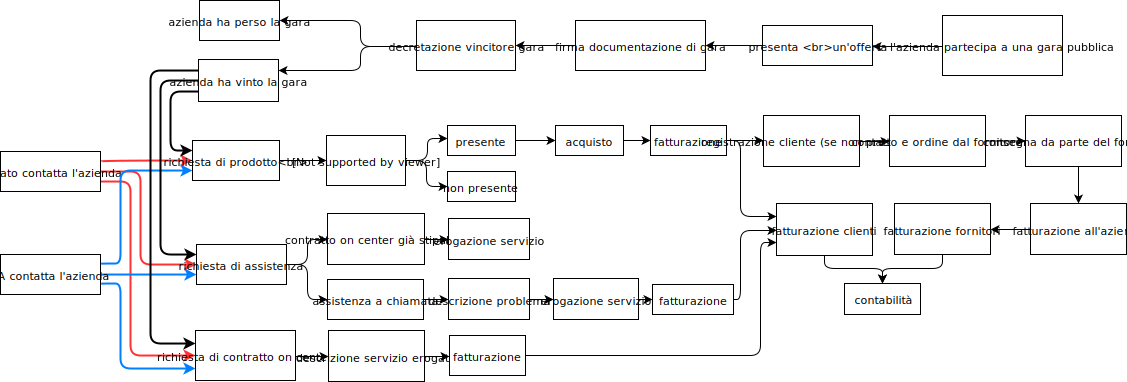
\includegraphics[width=\paperwidth-1cm, trim={0 8cm 0 0}, clip]{./immagini/processi_interni.pdf}}


% \newpage
%
% \begin{landscape} %inizia un foglio landscape
%
%
% %include un file pdf che contiene lo schema ruotato e dimensionato correttamente
% 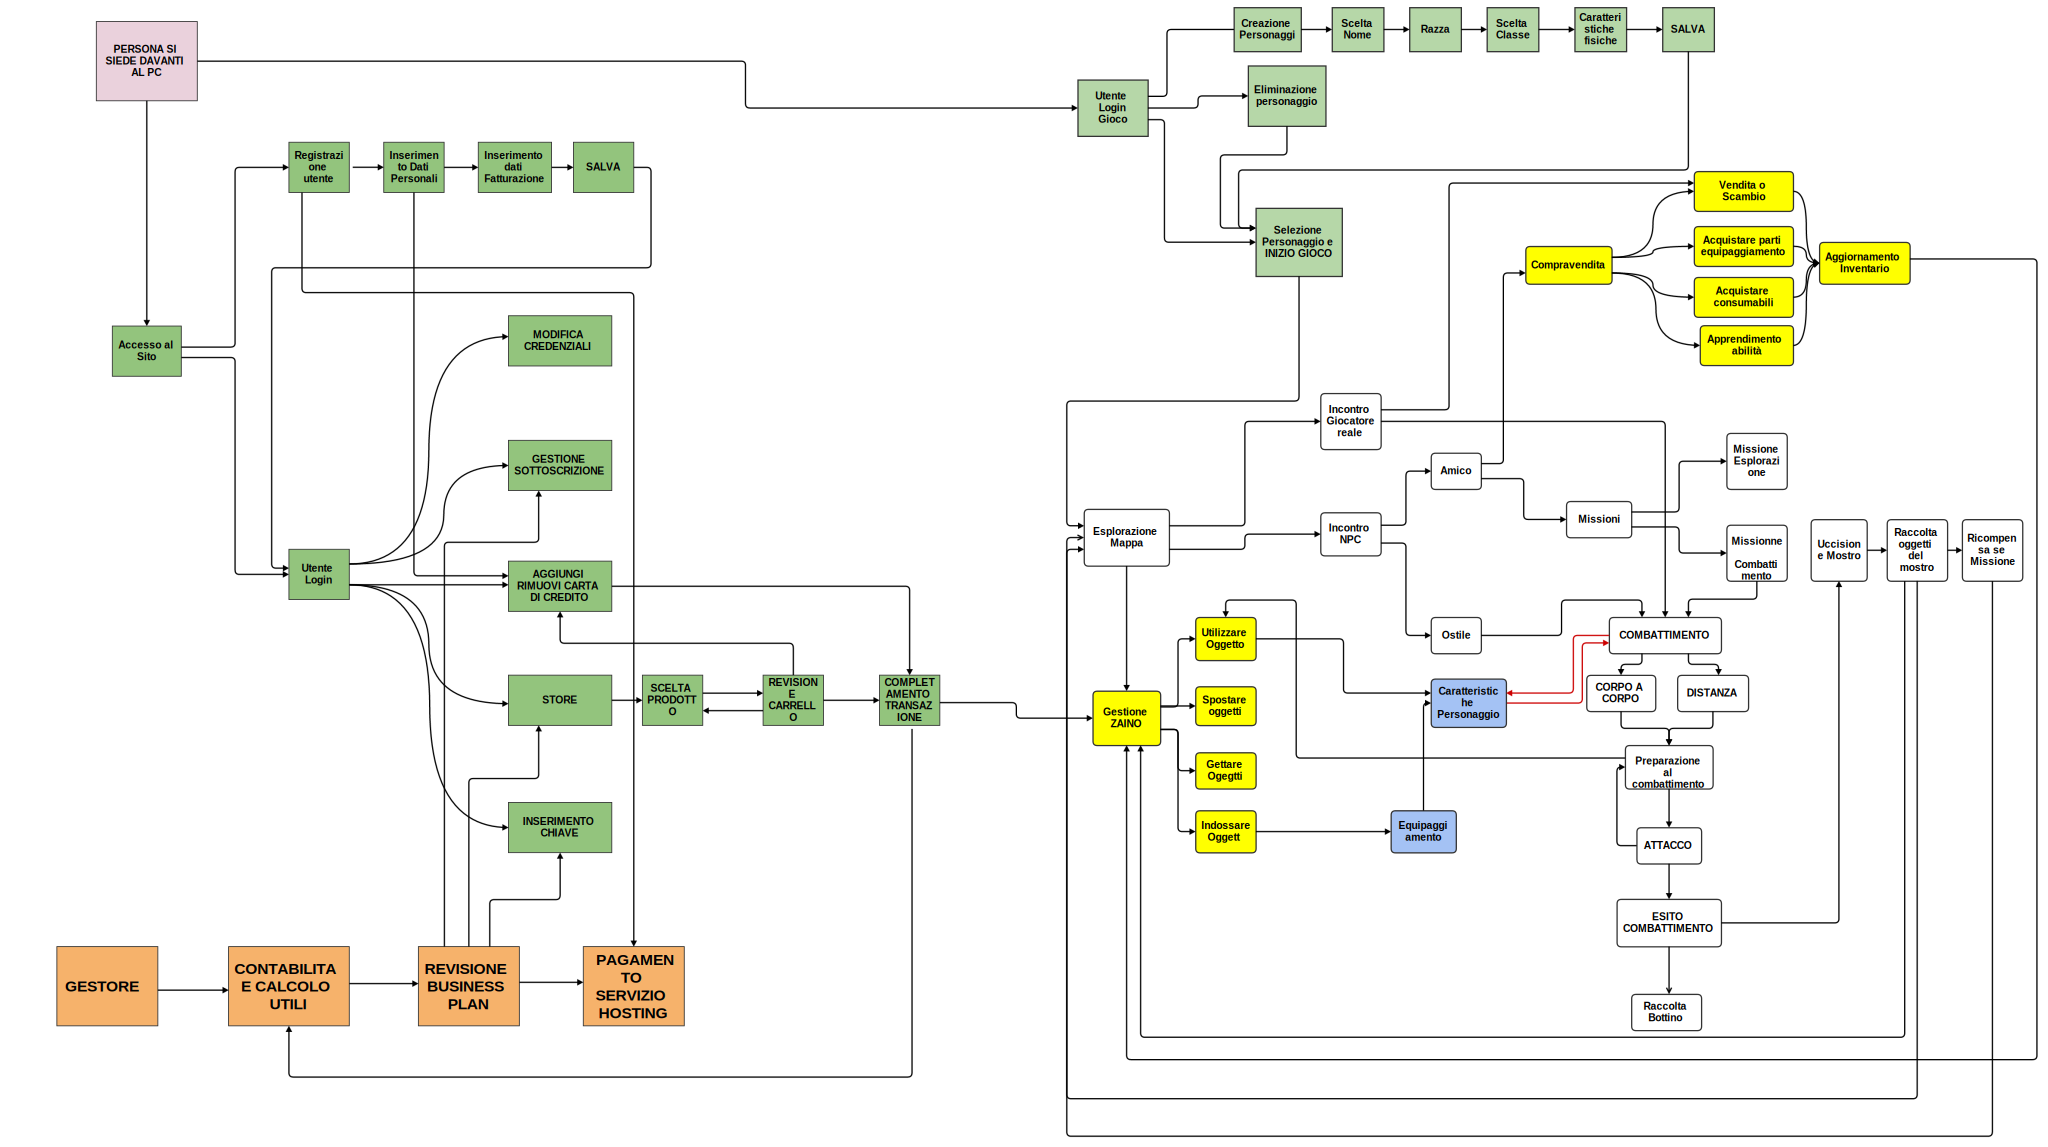
\includepdf[width=270mm, height=210mm, angle=90, keepaspectratio]{./pdf/sprocint.pdf}
%
% \end{landscape}


		%-----------------------------------------------------------------------
		\subsection{Requisiti Espressi nel Linguaggio Naturale}

		
Dopo aver analizzato le interviste effettuate e il diagramma  dei processi interni è stato possibile stabilire gli obbiettivi che  effettivamente vorremmo che la nostra base di dati raggiunga.
Lo scopo prefissato è pertanto realizzare una base di dati che sia di supporto a un gioco di ruolo online.
\\
Tale gioco è diviso in due parti: 
Il lato client che viene scaricato dall'utente sul PC e  che contiene il software di gioco; 
Il lato server  che si occupa di inviare/ricevere dati dal client. 
\\
La nostra base di dati è fondamentale per il funzionamento del gioco, quindi deve coesistere con esso per tutta la sua durata, garantire efficienza e risultare flessibile per successive aggiunte o modifiche delle modalità di gioco.
\\
Si dovranno gestire i dati relativi agli utenti, ai personaggi da essi creati, agli NPC , agli oggetti di gioco, alle abilità, e alle missioni.
Si necessita inoltre di memorizzare:

\begin{itemize}
\item	I prodotti che l'utente ha acquistato con valuta reale; 
\item	Le transazioni , riguardanti la compravendita di oggetti, che coinvolgono personaggi e/o NPC;
\item	Gli oggetti che il personaggio ha comprato;
\item	Gli oggetti che il personaggio indossa;
\item	Le abilità che il personaggio ha appreso;
\item	Le missioni che il personaggio ha accettato e lo stato delle stesse.
\end{itemize}

Per quel che riguarda gli \hl{utenti} sar\`{a} necessario sapere  l'user name e la password con i quali si sono iscritti al sito di gioco e i  dati relativi alla ragione sociale quindi nome, cognome, indirizzo e indirizzo e-mail. Si dovr\`{a} inoltre immagazzinare il codice di una o pi\`{u} carte di credito dell' utente, indispensabili per il  pagamento della sottoscrizione mensile o di eventuali espansioni o pacchetti oggetto.

Le sottoscrizioni e i pacchetti oggetti, come le espansioni saranno definite con le relative caratteristiche come livello massimo per le espansioni, la durata per le sottoscrizioni, e dovranno essere elencati gli oggetti dei vari pacchetti oggetti.\\

Ogni utente pu\'{o} poi creare pi\`{u} \hl{personaggi}. Di questi si necessita conoscere il nome che deve essere univoco e composto solamente da caratteri letterali, la razza che l'utente pu\`{o} scegliere fra elfo, nano e umano e la classe di gioco che deve essere una fra arciere, guerriero e mago, tenendo per\`{o} conto  che un nano potr\`{a} essere solo un arciere o un guerriero, un elfo potr\`{a} essere solo un arciere o un mago mentre un umano potr\`{a} sceglier fra  tutte e tre le opzioni. L'utente deve inoltre scegliere alcuni attributi fisici quali capelli, volto, barba e colore della pelle. Con la creazione al personaggio vengono assegnati un livello e dei punti esperienza. Vengono anche  fissati  alcune parametri o per meglio dire  \hl{statistiche} quali punti vita, punti mana, punti d'attacco, punti di difesa, forza, intelligenza e destrezza. Tali attributi influiscono sull'esito delle battaglie pertanto il giocatore avr\'{a} interesse, col progredire del gioco, a cercare di incrementarli al massimo. Un modo per far ci\'{o} consiste nell'acquisire pi\`{u} esperienza possibile. Infatti raggiunto un determinato quantitativo di \hl{esperienza} il personaggio sale di \hl{livello} e a ci\'{o} segue un aumento delle statistiche precedentemente citate. 
Di ogni personaggio sar\'{a} poi importante registrare la posizione sulla mappa nella quale si trova quando l'utente decide di uscire dal gioco in modo tale che da quella stessa posizione si possa poi riprendere quando il giocatore ri-effettuer\'{a} l'accesso.
\\
\\
Col naturale svolgersi  del gioco un personaggio  sarà portato a interagire con degli \hl{NPC (Non Playable Character)}. Questi sono personaggi gestiti dal computer e si distinguono in due grandi famiglie \hl{NPC amichevoli} e \hl{NPC ostili}. I primi sono in grado di aiutare il giocatore nel combattimento, di vendere o acquistare determinati oggetti o abilità al o dal personaggio e di assegnargli missioni. I secondi invece hanno lo scopo di combattere contro i personaggi.
Gli NPC hanno quindi un nome, un livello, una posizione nella quale è possibile trovarli dei punti di attacco e dei punti di difesa. Hanno poi a causa della distinzione precedentemente fatta alcune peculiarità dipendenti dal fatto che  siano essi amichevoli o ostili. Gli NPC ostili se sconfitti ci daranno una ricompensa sia in oggetti sia in esperienza che in  denaro.\\

Nel gioco è inserita una valuta fittizia l'oro il cui scopo è quello di permettere al personaggio di comperare oggetti.\\

Gli \hl{oggetti} si suddividono  in tre grandi categorie: 
\begin{itemize}
\item	oggetti equipaggiamento;
\item	oggetti consumabili;
\item	oggetti missione.
\end{itemize}

Gli \hl{oggetti equipaggiamento} servono nella fase di battaglia e per essere utilizzati hanno bisogno di essere indossati dal personaggio. Essi si dividono in armi: spade, asce, mazze, bastoni, bacchette, archi, balestre; e in armature: stivali, guanti, corazza, elmo. Le armature hanno tutte un ulteriore classificazione. A seconda del peso infatti si possono distinguere : armature leggere ,utilizzabili solo dagli arcieri, armature medie, utilizzabili solo dai maghi  e armature pesanti, utilizzabili solo dai guerrieri. Tutti gli equipaggiamenti hanno un nome, una descrizione  e  un livello che indica il livello minimo che deve avere il personaggio affinch\'{e} possa usare l'oggetto. Posseggono per di pi\`{u} dei punti d'attacco, dei punti di difesa, forza, destrezza e intelligenza  questi attributi in fase di battaglia si sommano a quelli del personaggio influendone sull'esito. Questi  oggetti, possono essere ottenuti acquistandoli da NPC o da altri personaggi o come ricompensa di  qualche missione e possono  essere venduti a NPC o a altri personaggi, hanno quindi un prezzo di acquisto e uno di vendita (solitamente inferiore).
\\

Gli \hl{oggetti consumabili} si dividono in pozioni curative e pozioni potenzianti. L'utilizzo permette di recuperare punti vita o punti mana per quel che riguarda le prime e di aumentare per un determinato periodo di tempo tutte o alcune statistiche le seconde. Anche i consumabili come gli equipaggiamento hanno un nome una descrizione e un livello. Identiche agli equipaggiamento sono le modalità di acquisto o vendita.\\

Gli \hl{oggetti missione} hanno un nome e una descrizione. All'interno del gioco hanno l'unica funzione di dover essere recuperati al fine di poter completare una missione (vedi missioni). Essi quindi non possono essere ne acquistati ne tanto meno indossati o usati.\\
Tutti gli oggetti una volta ottenuti finiscono nello zaino.\\

Ruolo di grande rilevanza durante la fase di battaglia è ricoperto dalle \hl{abilità}.
Ovvero tecniche speciali che per essere utilizzate hanno bisogno di punti mana e che  incrementano il valore di una o pi\`{u} statistiche del personaggio quali attacco, difesa, forza, destrezza e intelligenza. Ogni abilit\`{a} pu\`{o} essere utilizzata solo da personaggi aventi determinate classi di gioco e che hanno raggiunto determinati valori di livello.
\\
									
Come precedentemente accennato ogni personaggio pu\'{o} intraprendere una o pi\'{u} \hl{missioni} ,fino a un numero massimo stabilito dal gioco.
Le missioni , che vengono assegnate da un NPC, hanno un nome, una descrizione, e un livello. (inteso come livello che il personaggio deve avere per poter accettare la missione)
Abbiamo due tipi di missione: le missioni esplorazione e  le missioni combattimento. Le missioni esplorazione  consistono nel visitare determinate zone della mappa o recuperare determinati oggetti missione. Le missioni  combattimento riguardano l'abbattimento o il recupero di uno o pi\'{u} oggetti a seguito di una battaglia con un NPC ostile.
Qualsiasi  missione ha una \hl{ricompensa} sia in oro che in punti esperienza e talvolta anche in oggetti e per ottenerla \'{e} necessario, una volta raggiunti gli obiettivi della missione, ritornare dal NPC che la missione l'ha assegnata.\\

Si è detto che bisogna tener traccia delle \hl{transazioni} effettuate  dal personaggio. In particolare si vuole sapere quale oggetto viene acquistato o venduto, chi è l'acquirente e chi invece il venditore.
Tendendo presente inoltre che queste informazioni andranno perse una volta effettuato il logout da parte dell'utente.

\newpage 

		%------------------------------------------------
		\subsection{Glossario dei Termini}

		%Se non si vuole creare la tablella in latex è possibile farla con word, copincollarla
%nella sezione File/paste table data del sito http://www.tablesgenerator.com
%che genererà la tabella in latex
%non scordare di mettere le chiusure di table e di adjustbox

% Comando per fare le celle su più righe, separa ogni riga con '\\'
\newcommand{\specialcell}[2]{
  \begin{tabular}[c]{@{}l@{}}#1\end{tabular}}

\begin{table}[h!]
  \centering
  \begin{adjustbox}{width=\textwidth}
    \begin{tabular}{@{}llll@{}}
      \toprule
      \textbf{TERMINE} & \textbf{DESCRIZIONE} & \textbf{SINONIMI} & \textbf{COLLEGAMENTO} \\ \midrule

      \multicolumn{1}{|l|}{Utente}
      & \multicolumn{1}{l|}{\specialcell{Persona fisica che gestisce e gestisce \\ e controlla il personaggio.}}
      & \multicolumn{1}{l|}{Giocatore}
      & \multicolumn{1}{l|}{Personaggio} \\ \midrule

      \multicolumn{1}{|l|}{Utente}
      & \multicolumn{1}{l|}{Mufasa dio}
      & \multicolumn{1}{l|}{Giocatore}
      & \multicolumn{1}{l|}{Personaggio} \\ \midrule

      \multicolumn{1}{|l|}{Utente}
      & \multicolumn{1}{l|}{\specialcell{Persona fisica che gestisce e gestisce \\ e controlla il personaggio.}}
      & \multicolumn{1}{l|}{Giocatore}
      & \multicolumn{1}{l|}{Personaggio} \\ \midrule

      \multicolumn{1}{|l|}{Utente}
      & \multicolumn{1}{l|}{\specialcell{Persona fisica che gestisce e gestisce \\ e controlla il personaggio.}}
      & \multicolumn{1}{l|}{Giocatore}
      & \multicolumn{1}{l|}{Personaggio} \\ \midrule


    \end{tabular}
  \end{adjustbox}
\end{table}

		\newpage
		%------------------------------------------------
		\subsection{Eliminazione delle Ambiguit\'{a} Presenti}

		L'unica Ambiguit� presente sembra essere la definizione delle Statistiche del personaggio, che sono le stesse anche per gli NPC e per le abilit� che le modificano, per non fare confusione con la definizione di Attributo dei database abbiamo scelto di usare Statistiche.



		%------------------------------------------------
		\subsection{Strutturazione dei Requisiti}

		
\subsubsection{Frasi di Carattere Generale}
L'azienda necessita di interfacciarsi con diverse entità, fungendo da intermediaria indipendente, rispondendo alle richieste di gare pubbliche attraverso la disponibilità di fornitori privati. In tutto ciò la nostra base di dati può risultare fondamentale per l'ottimizzazione dei processi e in più per fornire importanti analisi su ciò che offre il mercato e quali migliorie possono essere apportate, così da ottimizzare non solo i processi, ma il business stesso.\newline
Si gestiranno perciò i dati riguardanti le gare pubbliche, i clienti, i fornitori, i prodotti, i servizi e tutte le tipologie di contratti stipulati tra l'azienda e i clienti.

\subsubsection{Frasi relative alle Gare Pubbliche}
Le gare pubbliche vengono pubblicate sul sito acquistinretepa.it, cioè il Portale degli acquisti della Pubblica Amministrazione di proprietà del Ministero dell'Economia e delle Finanze e del Consip.\newline
La sezione di interesse per l'azienda è quella del Mercato Elettronico delle Pubbliche Amministrazioni, chiamato MEPA. Qui le imprese possono vedere le gare pubbliche e parteciparvi.\newline
Un'azienda abilitata alla vendita sul MEPA, necessita di credenziali di accesso al sito suddetto, in questo modo può partecipare ad un numero illimitato di gare.\newline
L'iscrizione a una gara consiste nel effettuare un'offerta, e dalla richiesta di offerta possono essere ottenute tutte le informazioni sulla richiesta e il richiedente, cioè la pubblica amministrazione che ha eseguito la richiesta, con tanto di codice identificativo PA.\newline
Quindi è importante registrare tutte le informazioni. L'idea è quella di registrare non solamente le gare aggiudicate, ma anche quelle perse, in modo da poter effettuare delle analisi successive. La quantità di gare presenti permette di effettuare questo tipo di operazione manualmente. Potrebbe essere previsto un web scraper in fase avanzata che gestisca in automatico questa procedura.\newline
La registrazione è determinata da due fasi, quella iniziale in cui si accingono i dati generali sulla gara e sul cliente, e poi una fase finale, dopo la chiusura della gara, per raccogliere dati sugli aggiudicatari e l'offerta effettuata, sempre a scopo di analisi.

\subsubsection{Frasi relative ai Clienti}
Per quel che riguarda i clienti, si hanno sia enti privati che pubbliche amministrazioni. Per gli enti privati sono necessari i dati relativi alla ragione sociale, l'indirizzo, dati di fatturazione. Per le pubbliche amministrazioni, oltre a questi dati, servono informazioni riguardo al codice PA e all'indirizzo di posta PEC, tutte informazioni estraibili dalle richieste di offerta sul MEPA. \newline
Sia ai privati e sia alle pubbliche amministrazioni saranno poi legati i contratti e le fatture, nelle apposite tabelle.

\subsubsection{Frasi relative alle Assistenze}
Le assistenze si dividono in assistenze di due tipi:
\begin{itemize}
\item	assistenze on center;
\item	assistenze a chiamata;
\end{itemize}
Le assistenze on center sono erogate a domicilio, in seguito alla stipulazione di un contratto di durata prestabilita, solitamente dai quattro mesi a un anno, per cui il cliente paga una quota fissa in modo da ricevere assistenza sul luogo in base alle sue esigenze.\newline
I dati importanti al riguardo sono il costo del contratto, la data di inizio e la data di scadenza, e il tipo di assistenza.\newline
Le assistenze a chiamata non sono vincolate da uno contratto, il cliente può chiedere interventi su richiesta e paga a prestazione compiuta.
In questo caso si registrano la data in cui si è fatta assistenza, il tipo di servizio erogato, e il cliente che ha ricevuto assistenza.


\subsubsection{Frasi relative ai Prodotti}
I prodotti sono quelli messi a disposizione dai fornitori, i quali forniscono i propri cataloghi che comprendono una lista di codici prodotto con il relativo prezzo di vendita. I dati quindi da registrare sono soprattutto il codice prodotto, in quanto spesso i clienti chiedono un prodotto in base al codice specifico, e le caratteristiche tecniche del prodotto.\newline
In seguito alla vendita di un prodotto viene emessa una fattura al cliente con indicati i prodotti venduti, i costi, e i dati relativi a venditore e acquirente.

\subsubsection{Frasi relative ai Servizi}
I servizi sono entità particolari che necessitano di una standardizzazione nella loro trattazione in quanto il costo è molto variabile e non è determinato per forza in base al tempo speso per effettuare tale servizio. I servizi devono essere registrati con il loro costo, e deve essere strutturata una descrizione generica da poter riportare. Il servizio di per sè implica anche uno spostamento di cui tener conto, che potrebbe essere comparato a quelli che sono i costi di spedizione in caso di acquisto di un prodotto.\newline
Dopo l'erogazione di un servizio viene emessa una fattura al cliente che deve riportare la prestazione eseguita, il costo, e i dati relativi al fornitore e al ricevente del servizio.

\subsubsection{Frasi relative ai Fornitori}
I fornitori sono coloro da cui vengono acquistati i prodotti da vendere ai clienti. I dati necessari al riguardo sono simili a quelli dei clienti, quindi bisogna registrare ragione sociale, indirizzo, dati di fatturazione per i pagamenti. Ad essi è importante legare i catalogi forniti, che vengono consultati per verificare la disponibilità dei prodotti, e vengono aggiornati mensilmente.

\subsubsection{Frasi relative alle Fatture}
Si vogliono conoscere le informazioni relative a una fattura, sia in entrata che in uscita. Sono quindi necessari il codice del contratto a cui si riferisce, la data di emissione, la data entro cui è necessario pagare.

% \subsubsection{Frasi relative agli Ordini}
% Gli ordini rappresentano i prodotti acquistati dai fornitori. Spesso gli ordini effettuati non sono spediti all'azienda che deve poi spedirli ai clienti, ma vengono direttamente spediti al cliente, seguendo il modello di dropshipping. In ogni caso bisogna tener traccia anche dei costidi spedizone}, oltre che al prodotto interessato dall'ordine e le sue caratteristiche, il costo dell'ordine, il fornitore del prodotto, il cliente che ha acquistato il prodotto per cui è stato effettuato l'ordine. Tutto ciò implica la connessione di diverse entità interessate che insieme vanno a formare l'ordine. Qui come nelle trattative bisogna considerare la fattura, in particolare la fattura emessa ai clienti da parte della azienda, e in questo caso la fattura emessa dal fornitore all'azienda per l'acquisto.


		%------------------------------------------------
		\subsection{Specifica delle Operazioni}

		
% Calcoli fatti considerando una media di 3500 utenti connessi al server. Ad esclusione delle operazioni fatte ogni 3 anni che vengono svolte dagli sviluppatori al rilascio delle nuove espansioni. La 34,35,36 vengono fatte con le patch mensili per bilanciare il gioco.

Assumptions: Numero fornitori: 10

\begin{enumerate}

  \item Inserimento nuovo cliente (in media 10 volte al mese)
  \item Inserimento nuova gara pubblica (in media una volta al giorno)
  \item Inserimento nuova trattativa diretta (in media una volta a settimana)
  \item Inserimento nuovo prodotto (due volte al mese)
  \item Inserimento nuovo servizio (due volte all'anno)
  \item Inserimento nuovo contratto di assistenza on center (una volta al mese)
  \item Inserimento nuova fattura (in media tre volte al giorno)
  \item Inserimento nuovo fornitore (due volte all'anno)
  \item Inserimento di un nuovo catalogo (due volte all'anno)
  \item Inserimento nuova tabella di costi di spedizione (due volte all'anno)
  \item Aggiornamento di una gara pubblica in seguito alla sua chiusura (in media una volta al giorno)
  \item Aggiornamento di una trattativa diretta in seguito alla sua stipula (in media una volta a settimana)
  \item Aggiornamento di un catalogo (dieci volte al mese)
  \item Aggiornamento di una tabella di costi di spedizione (in media due volte all'anno)
  \item Modifica dati cliente (in media 20 volte all'anno)
  \item Modifica dati di un servizio (in media due volte all'anno)
  \item Modifica dati di un fornitore (in media tre volte all'anno)
  \item Cancellazione di un prodotto (quattro volte all'anno)
  \item Cancellazione di un servizio (in media una volta all'anno)
  \item Cancellazione di un fornitore (una volta all'anno)
  \item Cancellazione di un catalogo (una volta all'anno)
  \item Consultazione dati dei clienti (in media 10 volte al giorno)
  \item Consultazione dati dei fornitori (in media due volte al giorno)
  \item Consultazione contratti di assistenza on center (in media due volte a settimana)
  \item Consultazione contratti di assistenza on center in un determinato periodo (due volte al mese)
  \item Consultazione dati di una gara pubblica (in media cinque volte al giorno)
  \item Consultazione dati di una trattativa diretta (in media due volte al giorno)
  \item Consultazione caratteristiche di un prodotto (cinque volte al giorno)
  \item Consultazione prezzo di un prodotto (dieci volte al giorno)
  \item Consultazione di una fattura (una volta al giorno)
  \item Statistica delle gare pubbliche vinte e perse in un determinato periodo (una volta al mese)
  \item Statistica delle trattative dirette stipulate (una volta al mese)
  \item Statistica dei prodotti più venduti (una volta al mese)
  \item Statistica dei servizi più erogati (una volta al mese)
  \item Verifica del pagamento delle fatture da parte dei clienti (due volte a settimana)
  \item Verifica di scadenza imminente del pagamento delle fatture da parte dei clienti (tre volte al mese)
  \item Verifica del pagamento delle fatture da parte dell'azienda (due volte a settimana)
  \item Verifica di scadenza imminente del pagamento delle fatture da parte dell'azienda (tre volte al mese)
  \item Calcolo del guadagno netto ad una certa data (una volta al mese)
  \item Calcolo del volume di vendite in un determinato periodo (una volta al mese)
  \item Calcolo dei costi di spedizione di un'acquisto (tre volte al giorno)
  \item Selezione della migliore combinazione di prodotti (tre volte al giorno)
  \item Selezione che tiene conto dei margini di guadagno e dei volumi (si può fare?) Considerare margini (standard: 10%, ma si può abbassare) ()

\end{enumerate}


% 		\newpage
% %------------------------------------------------
% 	\section{Progettazione Concettuale}
%
%
% 		\subsection{Strategia di Progetto }
% 			Svilupperemo lo schema concettuale con un approccio misto, cio� partiremo da dei concetti astratti principali che descrivono le specifiche in modo blando e andremo a raffinarli (strategia top-down), procederemo nella raffinazione fino ad arrivare ad un soddisfacente grado di dettaglio per poi correggere lo schema secondo una strategia inside-out.
%
%
% 		%------------------------------------------------
% 		\subsection{Individuazione Entit\'{a} e Relazioni Principali}
%
% 		Come precedentemente specificato sono state estrapolate le entità principali intorno alle quali sviluppare la progettazione. Ciò è stato possibile grazie ad un'approfondita analisi del flusso aziendale, derivato direttamente dall'analisi delle azioni e dei processi interni.\newline
Il risultato è dato dalle cinque seguenti entità fondamentali: \newline

\noindent\makebox[\textwidth]{\includegraphics[width=\textwidth-5cm]{./immagini/entita_fondamentali.pdf}}
\newline
\newline
RICHIESTA SUL MEPA: il blocco rappresenta gli strumenti che le pubbliche amministrazioni utilizzano per  l'interfacciamento con la nostra azienda. In questo caso si parla di gare pubbliche oppure richieste di trattativa dirette. \newline
PA, AZIENDA O PERSONA: è il macrogruppo comprensivo delle persone giuridiche che hanno rapporti commerciali con la nostra azienda, tra questi ci sono i fornitori e i clienti, sia privati e pubbliche amministrazioni.\newline
PRODOTTO O SERVIZIO: comprende tutti i prodotti vendibili o acquistabili dall'azienda disponibili dai fornitori e i servizi disponibili.\newline
FATTURA: è l'entità fondamentale che interviene in tutte le operazioni sia per l'acquisto che per la vendita di prodotti e/o servizi.

\newpage

%
% 		%------------------------------------------------
% 		\begin{landscape}
%
% 		\subsection{Scheletro dello Schema ER}
% 			Possiamo unire le Componenti principali nel seguente schema scheletro:
%
% 			\begin{figure}[H]
% 			\centering
% 			\includegraphics[width=\linewidth]{./immagini/SCHEMASCHELETRO.png}
% 		\end{figure}
%
% 		\end{landscape}
%
% \newpage
% 		%------------------------------------------------
% 		\subsection{Sviluppo delle Componenti dello Schema}
%
% 		\subsubsection{RICHIESTA SUL MEPA}
bla bla bla
\includegraphics[width=0.7\linewidth]{./immagini/richiesta_sul_mepa.pdf}

\subsubsection{PA O PERSONA O AZIENDA}
bla bla bla
\includegraphics[width=0.7\linewidth]{./immagini/pa_persona_o_azienda.pdf}

\subsubsection{PRODOTTO O SERVIZIO}
bla bla bla
\includegraphics[width=0.7\linewidth]{./immagini/prodotto_servizio.pdf}

\subsubsection{FATTURA}
bla bla bla
\includegraphics[width=0.7\linewidth]{./immagini/fattura.pdf}



% Procediamo ora secondo la strategia Top-down raffinando le definizioni delle entità e aggiungendo ulteriori relazioni.
% \subsubsection{Personaggio}
% Sappiamo che il personaggio ha parecchie caratteristiche e valori che lo contraddistinguono, possiamo suddividerle in 4 gruppi:
% Posizione, Fisico, Statistiche e Statistiche totali
%
% \begin{figure}[H]
% \centering
% \includegraphics[width=0.7\linewidth]{./immagini/personaggiodef.png}
% \end{figure}
%
% \newpage
%
%
% \subsubsection{NPC}
% Gli npc sono divisi principalmente in ostili e amichevoli, questo ne determina fortemente la funzione all'interno del gioco, le relazioni con le altre entità nonchè i dati stessi che essi utilizzano, è quindi necessaria una Generalizzazione che i suddivida di conseguenza
%
% \begin{figure}[H]
% \centering
% \includegraphics[width=0.7\linewidth]{./immagini/npcdef.png}
% \end{figure}
%
%
% \subsubsection{Oggetto}
% Per gli oggetti sappiamo che alcuni di essi possono essere equipaggiati, consumati dal personeggio oppure essere oggetti missione, questo fatto oltre a comportare una Generalizzazione implica la necessità di una relazione di equipaggiamento, una di consumo e una di stock per descrivere la proprietà di un OGGETTO da parte di un PERSONAGGIO
%
% \begin{figure}[H]
% \centering
% \includegraphics[width=0.7\linewidth]{./immagini/oggettodef.png}
% \end{figure}
%
%  \newpage
%
% \subsubsection{Abilità}
% Dalle interviste sappiamo che le abilità hanno svariati attributi che sono poi i valori da sommare alle statistiche dei personaggi che imparano le abilità, hanno anche un costo e un livello massimo.
%
% \begin{figure}[H]
% \centering
% \includegraphics[width=0.7\linewidth]{./immagini/ABILITADEF.png}
% \end{figure}
%
% \subsubsection{Transazione}
% Le transazioni saranno necessarie solo per tenere traccia degli acquisti della sessione, esse avranno un SOGGETTO e un OGGETTO intesi come "chi vende a chi compra"
%
% \begin{figure}[H]
% \centering
% 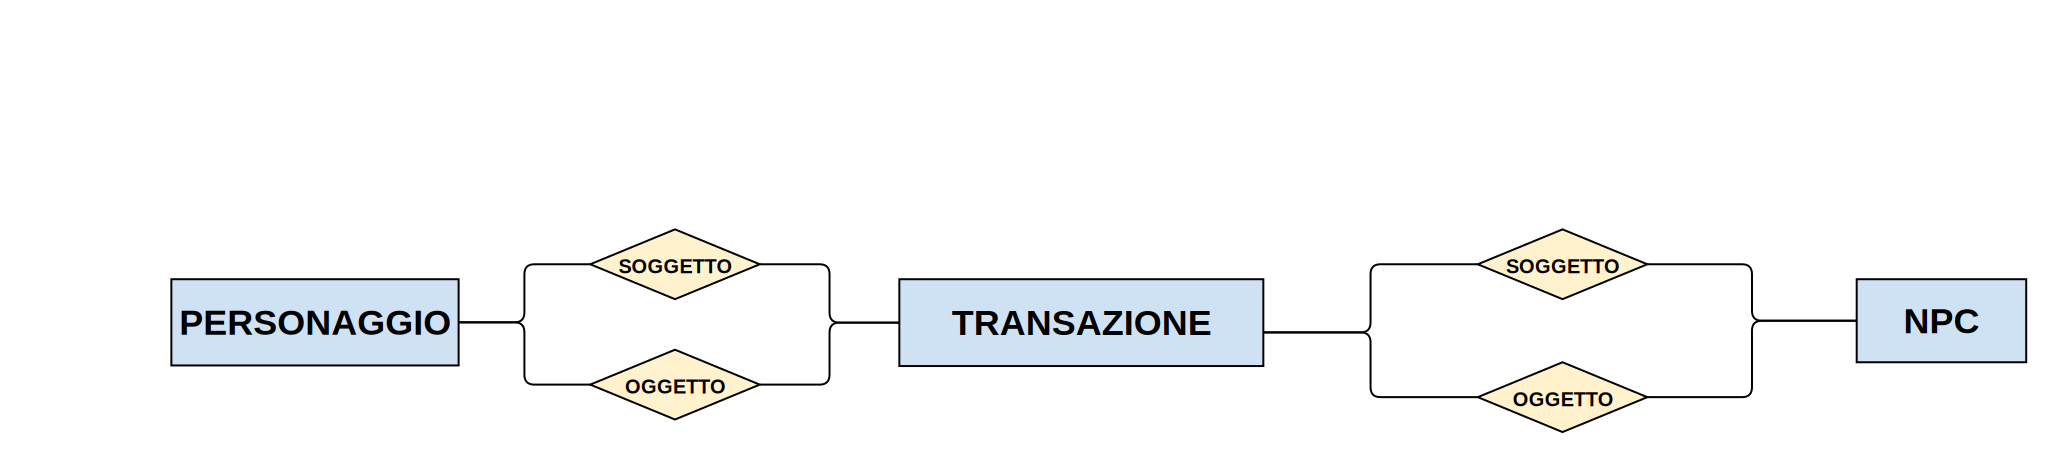
\includegraphics[width=0.7\linewidth]{./immagini/TRANSAZ.png}
% \end{figure}
% AMBIGUITA
%
% \subsubsection{Utente}
% L'utente è la persona vera e propria che si logga per giocare con uno dei suoi personaggi, puo fare acquisti nello Store con una delle sue carte di credito, eliminare o creare personaggi e modificare i suoi dati di fatturazione.
%
%
% \begin{figure}[H]
% \centering
% \includegraphics[width=0.7\linewidth]{./immagini/untentedef.png}
% \end{figure}
%
% \subsubsection{Prodotto}
% I PRODOTTI nel nostro gioco sono principalmente 3, cioè le SOTTOSCRIZIONI, I PACCHETTI OGGETTI che permettono di acquistare un gruppo di oggetti Elencati e le ESPANSIONI del Gioco che permettono di raggiungere un livello massimo piu alto.
%
% \begin{figure}[H]
% \centering
% \includegraphics[width=0.7\linewidth]{./immagini/prodottodef.png}
% \end{figure}
%
% \newpage

%
% 			\subsubsection{Raffinamenti successivi}
%
% 				Per la Relazione di CONSUMO dell'OGGETTO da parte del PERSONAGGIO abbiamo riscontrato un problema, il consumo �  un azione che � possibile ripetere nel corso del tempo per lo stesso oggetto, ci� risulta incompatibile con la nostra definizione di consumo come relazione, � stato quindi necessario Reificare la relazione in un entit� CONSUMO e due relazioni CONSUMANTE e CONSUNTO.

\begin{figure}[H]
\centering
\includegraphics[width=0.4\linewidth]{./immagini/personaggioconsumabili.png}
\end{figure}

\begin{figure}[H]
\centering
\includegraphics[width=0.8\linewidth]{./immagini/MISSIONEOBIETTIVI.png}
\end{figure}



\begin{landscape} %inizia un foglio landscape

%include un file pdf che contiene lo schema 
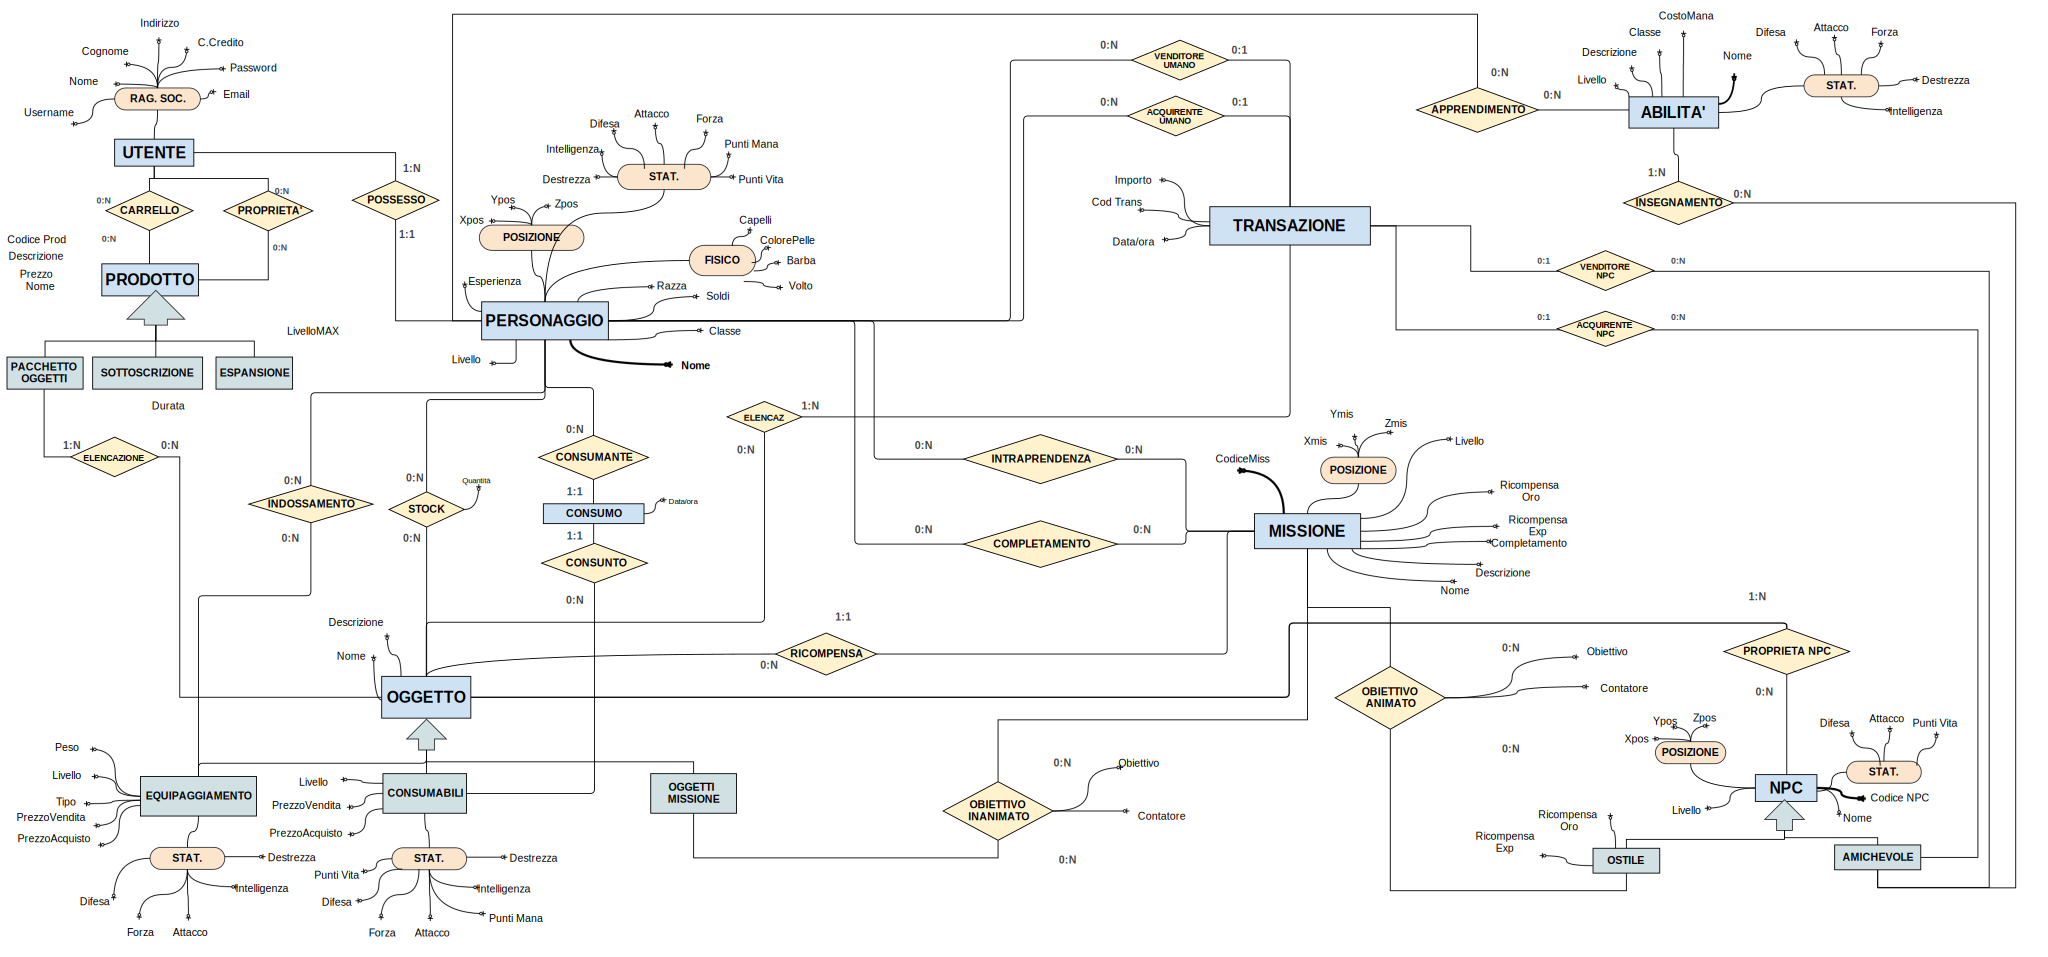
\includepdf[width=270mm, height=210mm, angle=90, keepaspectratio]{./pdf/sbizz.pdf}

\end{landscape}
%
% 		%------------------------------------------------
% 		\subsection{Analisi Qualitativa dello Schema ER}
%
% 		In questa fase si effettua un'analisi delle qualità dello schema appena definito. Si suddividono in quattro categorie:
\begin{itemize}
\item \textbf{Correttezza:} Le entità sono usate in maniera consona e congruente per il loro scopo e non risultano errori sintattici e semantici.
\item \textbf{Completezza:} Il flusso di informazioni relativo ai processi interni dell'azienda è ben rappresentato dal modello. Questo significa che lo schema è completo e rappresenta i processi interni in maniera fedele rendendo naturale il percorso logico rappresentato.
\item \textbf{Leggibilità:} Lo schema presenta una buona complessità concentrata maggiormente nella regione centrale. Nonostante ciò il flusso di informazioni risulta spontaneo quindi la comprensibilità dello schema non è compromessa anche se sono stati necessari alcuni incroci per ottimizzare la disposizione di tutti i componenenti.
 \item \textbf{Minimalità:} Ogni specifica è utilizzata una sola volta all'interno dello schema quindi esso non contiene ridondanze.
\end{itemize}

%
% 		%------------------------------------------------
% 		\subsection{Dizionario Dei Dati}
%
% 			\subsubsection{Entit�}
%
% 				
\begin{table}[H]
\resizebox{\textwidth}{!}{%
\begin{tabular}{|l|l|l|l|}
\hline
\textbf{Nome Entit�} & \textbf{Descrizione}                                                                                                                                                                             & \textbf{Attributi}                                                                                                                                                                                                                                                                                                                                                                                                                     & \textbf{Identificatore}                                                                                                                                                                                                                                                                                                                  \\ \hline
Utente               & Fruitore finale del gioco                                                                                                                                                                        & \begin{tabular}[c]{@{}l@{}}username (stringa),  nome (stringa), cognome (stringa),\\  indirizzo (stringa), password (stringa), email (stringa)\end{tabular}                                                                                                                                                                                                                                                                            & Username (stringa)                                                                                                                                                                                                                                                                                                                       \\ \hline
Prodotto             & \begin{tabular}[c]{@{}l@{}}Tutto ci� nell'ambito del gioco\\ che l'utente pu� acquistare\\ con valuta reale.\\  Comprende le entit� Sottoscrizione, \\ PacchettoOggetti, Espansione.\end{tabular} & \begin{tabular}[c]{@{}l@{}}Codice (numerico),nome(stringa)\\  descrizione (stringa), prezzo (numerico)\end{tabular}                                                                                                                                                                                                                                                                                                                    & Codice (numerico)                                                                                                                                                                                                                                                                                                                        \\ \hline
Sottoscrizione       & \begin{tabular}[c]{@{}l@{}}� un prodotto, abbonamento mensile\\  del gioco\end{tabular}                                                                                                          & ? Codice (numerico), durata (numerico)                                                                                                                                                                                                                                                                                                                                                                                                 & "                                                                                                                                                                                                                                                                                                                                        \\ \hline
PacchettoOggetti     & \begin{tabular}[c]{@{}l@{}}sono un prodotto, \\ particolari oggetti \\ destinati all'abbellimento\\  del personaggio\end{tabular}                                                                & ? Codice (numerico)                                                                                                                                                                                                                                                                                                                                                                                                                    & "                                                                                                                                                                                                                                                                                                                                        \\ \hline
Espansione           & \begin{tabular}[c]{@{}l@{}}Sono un prodotto, \\ aggiunte al gioco \\ rilasciate a cadenza triennale\\ comprendono nuove missioni e/o \\ nuovi oggetti e/o nuovi NPC\end{tabular}                   & \begin{tabular}[c]{@{}l@{}}??livello massimo? indica il nuovo livello massimo \\ che il personaggio potr� raggiungere.\\ Codice (numerico), livello massimo (numerico)\end{tabular}                                                                                                                                                                                                                                                    & "                                                                                                                                                                                                                                                                                                                                        \\ \hline
Personaggio          & \begin{tabular}[c]{@{}l@{}}Alter ego creato dall'utente\\  per poter giocare\end{tabular}                                                                                                        & \begin{tabular}[c]{@{}l@{}}Nome (stringa), razza (stringa), classe (stringa),\\  livello (numerico), esperienza (numerico), \\ soldi (numerico), capelli (stringa),\\  colorePelle (stringa), barba (stringa), \\ volto (stringa), puntiVita (numerico),\\  puntiMana(numerico), forza (numerico),\\  destrezza (numerico), intelligenza (numerico),\\  xPos (numerico), yPos (numerico), zPos (numerico) nomeUt(stringa)\end{tabular} & \begin{tabular}[c]{@{}l@{}}?razza? � una caratteristica del\\ personaggio e influenza ?classe?\\e le statistiche\\  (?forza?, ?destrezza?, ?intelligenza?).\\ ?capelli?, ?colorePelle?, \\ ?barba?, \\ ?volto? corrispondono ad oggetti \\ grafici del software di gioco.\\ ?xPos?, ?yPos?, ?zPos?\\ cordinate del personaggio\end{tabular} \\ \hline
Transazione          & \begin{tabular}[c]{@{}l@{}}Resoconto degli oggetti acquistati\\ dal personaggio in una sessione di gioco\end{tabular}                                                                            & \begin{tabular}[c]{@{}l@{}}Codice (numerico), dataOra (time), \\ importo (numerico), compratoreReale (stringa),\\  venditoreReale (stringa), compratorePC (stringa),\\  venditorePC (stringa)\end{tabular}                                                                                                                                                                                                                             & \begin{tabular}[c]{@{}l@{}}?dataOra? indica l'orario in cui\\  � stata effettuata la transizione.\\  ?CompratoreReale?,  ?compratorePC?\\ ci dice se chi compra\\  � un personaggio o un NPC.\\  ?venditoreReale?, ?venditorePC? ci dice se\\  chi vende � un personaggio\\ o un NPC\end{tabular}                                            \\ \hline
Consumo              & \begin{tabular}[c]{@{}l@{}}Resoconto degli oggetti\\  consumabili utilizzati dall utente\end{tabular}                                                                                            & Codice ( numerico), data(time)                                                                                                                                                                                                                                                                                                                                                                                                         & ?                                                                                                                                                                                                                                                                                                                                        \\ \hline
Oggetto              & \begin{tabular}[c]{@{}l@{}}Strumenti acquisibili nel gioco.\\  Comprende Equipaggiamento, \\ Consumabili, OggettiMissione\end{tabular}                                                           & Nome (stringa), descrizione (stringa)                                                                                                                                                                                                                                                                                                                                                                                                  & Nome (stringa)                                                                                                                                                                                                                                                                                                                           \\ \hline
Equipaggiamento      & \begin{tabular}[c]{@{}l@{}}Tipologia di oggetto. Strumenti con\\  effetto permanente che influenzano\\  la battaglia.\end{tabular}                                                               & \begin{tabular}[c]{@{}l@{}}nome (stringa), livello ( numerico),\\  tipo (stringa), peso (stringa), attacco (numerico),\\  difesa (numerico), forza(numerico), destrezza (numerico),\\  intelligenza (numerico), prezzoVendita (numerico),\\  prezzoAcquisto(numerico)\end{tabular}                                                                                                                                                     & \begin{tabular}[c]{@{}l@{}}?tipo? specifica se un equipaggiamento \\ � un arma o un armatura.\\ Il ?peso? di un equipaggiamento\\  determina la razza del\\ personaggio che potr� adoperarlo.\end{tabular}                                                                                                                                 \\ \hline
Consumabili          & \begin{tabular}[c]{@{}l@{}}Tipologia di oggetto.\\Strumenti con effetto temporaneo \\ che influenzano la battaglia\end{tabular}                                                                    & \begin{tabular}[c]{@{}l@{}}nome (stringa), livello ( numerico), puntiVita (numerico),\\ puntiMana (numerico), attacco (numerico), difesa (numerico),\\  forza(numerico), destrezza (numerico), intelligenza (numerico),\\  prezzoVendita (numerico), prezzoAcquisto(numerico),durata(intero)\end{tabular}                                                                                                                             &                                                                                                                                                                                                                                                                                                                                          \\ \hline
OggettiMissione      & \begin{tabular}[c]{@{}l@{}}Tipologia di oggetto il cui scopo\\  � il ritrovamento al fine di completare\\  missioni\end{tabular}                                                                 & Nome (stringa)                                                                                                                                                                                                                                                                                                                                                                                                                         & ?                                                                                                                                                                                                                                                                                                                                        \\ \hline
Missione             & \begin{tabular}[c]{@{}l@{}}Incarico che il personaggio svolge\\  per ottenere esperienza e denaro.\end{tabular}                                                                                  & \begin{tabular}[c]{@{}l@{}}Codice (numerico), nome (stringa), descrizione ( stringa), livello (numerico),\\  completamento(numerico),\\  ricompensaOro (numerico), ricompensaExp (numerico),\\  xMiss (numerico), yMiss (numerico), zMiss (numerico)\end{tabular}                                                                                                                                                                      & Codice (numerico)                                                                                                                                                                                                                                                                                                                        \\ \hline
Abilit�              & \begin{tabular}[c]{@{}l@{}}Tecnica di combattimento che\\ il personaggio usa in battaglia.\end{tabular}                                                                                          & \begin{tabular}[c]{@{}l@{}}Nome (stringa), descrizione (stringa), classe (stringa), livello (numerico),\\  costoMana (numerico), \\ attacco (numerico), difesa (numerico), forza(numerico), destrezza (numerico), \\ intelligenza (numerico), prezzo(numerico)\end{tabular}                                                                                                                                                            & Nome (stringa)                                                                                                                                                                                                                                                                                                                           \\ \hline
NPC                  & \begin{tabular}[c]{@{}l@{}}Personaggio gestito dal computer.\\  Si distingue in NPCAmichevole \\ e NPCOstile.\end{tabular}                                                                       & \begin{tabular}[c]{@{}l@{}}Nome (stringa), livello (numerico), puntiVita (numerico), attacco (numerico), \\ difesa (numerico), xPos (numerico), yPos (numerico), zPos (numerico)\end{tabular}                                                                                                                                                                                                                                          & ?                                                                                                                                                                                                                                                                                                                                        \\ \hline
NPCAmichevole        & \begin{tabular}[c]{@{}l@{}}NPC che aiuta il personaggio vendendogli\\ abilit� e oggetti o combattendo\\  al suo fianco\end{tabular}                                                              & ?                                                                                                                                                                                                                                                                                                                                                                                                                                      & ?                                                                                                                                                                                                                                                                                                                                        \\ \hline
NPCOstile            & NPC che combatte contro il personaggio                                                                                                                                                           & \begin{tabular}[c]{@{}l@{}}?\\ Codice (numerico)\end{tabular}                                                                                                                                                                                                                                                                                                                                                                          &                                                                                                                                                                                                                                                                                                                                          \\ \hline
Carta credito        & Elenco delle carte di credito degli utenti                                                                                                                                                       & numero(numerico),cvv(numerico),scadenza(date)                                                                                                                                                                                                                                                                                                                                                                                          &                                                                                                                                                                                                                                                                                                                                          \\ \hline
\end{tabular}
}
\end{table}


% 		%------------------------------------------------
% 		\subsection{Regole Di Vincolo}
%
% 		
\begin{itemize}
\item Gli NPc insegnanti insegna no le abilit\'{a} scelte per loro dal programmatore
\item Non tutti gli ogggetti possono essere venduti da un NPC ma ogni oggetto pu\`{o} essere venduto a un npc
\item La durata della sottoscrizione \'{e} in mesi
\item La durata dei consumabili \'{e} minuti
\item Il livello del personaggio, di defailt \`{e} 1
\item Le armi non hanno peso


\end{itemize}
% 		%------------------------------------------------
% 		\subsection{Vincoli Non Esprimibili}
%
% 		
\begin{itemize}
\item Npc non vende a npc
\item Gli Oggetti missione non si vendono
\item Oggetti missione non possono essere ricompense missioni
\item una transazione non puo' avere due relazioni Soggetto o Oggetto
\item La classe \'{e} vincolata alla razza
\end{itemize}
%
% %------------------------------------------------
%
% 	\section{Progettazione Logica}
%
% 		\subsection{Tavola dei Volumi e Delle Operazioni}
%
% 		

\subsubsection{Tavola dei Volumi}

Il gioco in questione \'{e} in fase di progettazione, quindi i volumi delle entit\'{a} e delle relazioni sono stati individuati su una stima di mercato,che prevede il raggiungimento dei valori proposti entro i primi tre mesi di gioco. Solitamente in questo periodo si ha il boom di iscrizioni ad un gioco online, che poi vanno a diminuire di molto nel tempo cos\`{\i}come l'attività dei giocatori. I dati indicati con (**) variano velocemente nel tempo e sono pertanto molto indicativi. 

\begin{table}[H]
\centering

\resizebox{0.7\textwidth}{!}{%
\begin{tabular}{|l|l|l|}
\hline
\textbf{CONCETTO}                & \textbf{TIPO} & \textbf{VOLUME}           \\ \hline
Utente                           & E             & 5000                      \\ \hline
Personaggio                      & E             & 10000                     \\ \hline
Missione                         & E             & 500                       \\ \hline
Abilità                          & E             & 30                        \\ \hline
Oggetto                          & E             & 1000                      \\ \hline
Equipaggiamento                  & E             & 400                       \\ \hline
Consumabili                      & E             & 100                       \\ \hline
Oggetti Missione                 & E             & 500                       \\ \hline
Consumo                          & E             & 100000**                  \\ \hline
Npc Amichevole                   & E             & 750                       \\ \hline
Npc Ostile                       & E             & 1000                      \\ \hline
Transazione                      & E             & 120000**                  \\ \hline
Prodotto                         & E             & 50                        \\ \hline
Sottoscrizione                   & E             & 3                         \\ \hline
Pacchetto Oggetti                & E             & 46                        \\ \hline
Espansione                       & E             & 1                         \\ \hline
Indossamento                     & R             & 14000**                   \\ \hline
Stock                            & R             & 160000                    \\ \hline
Intraprendenza                   & R             & 25000                     \\ \hline
Completamento                    & R             & 10000                     \\ \hline
Obiettivo animato                & R             & 300                       \\ 
\end{tabular}
}
\end{table}
\newpage

\begin{table}[H]
\centering
\resizebox{0.7\textwidth}{!}{%
\begin{tabular}{|l|l|l|}
Obiettivo inanimato              & R             & 400                       \\ \hline
Ricompensa                       & R             & 700                       \\ \hline
Proprietà NPC Amichevole         & R             & 18750                     \\ \hline
Proprietà NPC Ostile             & R             & 4000                      \\ \hline
Apprendimento                    & R             & 50000                     \\ \hline
Insegnamento                     & R             & 5000                      \\ \hline
Possesso                         & R             & 15000                     \\ \hline
Carrello                         & R             & 25000                     \\ \hline
Proprietà                        & R             & 50000                     \\ \hline
Elencazione Pacchetto Oggetti                     & R             & 184  \\ \hline
Elencazione Transazione                          & R             & 120000                          \\ \hline
Consumante                       & R             & 100000**                  \\ \hline
Consunto                         & R             & 100000**                  \\ \hline
Compratore Personaggio           & R             & 90000                           \\ \hline
Venditore Personaggio            & R             & 30000                          \\ \hline
Compratore NPC                   & R             & 30000                          \\ \hline
Venditore NPC                    & R             & 90000                          \\ \hline
Specificazione Sottoscrizione    & R             & 3                         \\ \hline
Specificazione Pacchetto Oggetti & R             & 46                        \\ \hline
Specificazione Espansione        & R             & 1                         \\ \hline
Specificazione Equipaggiamento   & R             & 400                       \\ \hline
Specificazione Consumabili       & R             & 100                       \\ \hline
Specificazione Oggetto Missione  & R             & 500                       \\ \hline
\end{tabular}
}
\end{table}

\subsubsection{Tavola Operazioni}


\begin{table}[H]
\centering
\resizebox{0.5\textwidth}{0.48\textheight}{%
\begin{tabular}{ll}
\hline
\textbf{OPERAZIONE}      & \textbf{FREQUENZA}                           \\ \hline
\multicolumn{1}{|l|}{1}  & \multicolumn{1}{l|}{2 volte al giorno}       \\ \hline
\multicolumn{1}{|l|}{2}  & \multicolumn{1}{l|}{5 volte al giorno}       \\ \hline
\multicolumn{1}{|l|}{3}  & \multicolumn{1}{l|}{175 volta ogni 3 anni}   \\ \hline
\multicolumn{1}{|l|}{4}  & \multicolumn{1}{l|}{200 volte ogni 3 anni}   \\ \hline
\multicolumn{1}{|l|}{5}  & \multicolumn{1}{l|}{100 volte ogni 3 anni}   \\ \hline
\multicolumn{1}{|l|}{6}  & \multicolumn{1}{l|}{35000 volte al giorno}   \\ \hline
\multicolumn{1}{|l|}{7}  & \multicolumn{1}{l|}{21000 volte al giorno}   \\ \hline
\multicolumn{1}{|l|}{8}  & \multicolumn{1}{l|}{10 volte ogni 3 anni}    \\ \hline
\multicolumn{1}{|l|}{9}  & \multicolumn{1}{l|}{2 volte a settimana}     \\ \hline
\multicolumn{1}{|l|}{10} & \multicolumn{1}{l|}{70000 volte al giorno}   \\ \hline
\multicolumn{1}{|l|}{11} & \multicolumn{1}{l|}{200000 volte al giorno}  \\ \hline
\multicolumn{1}{|l|}{12} & \multicolumn{1}{l|}{17500 volte al giorno}   \\ \hline
\multicolumn{1}{|l|}{13} & \multicolumn{1}{l|}{100000 volte al giorno}  \\ \hline
\multicolumn{1}{|l|}{14} & \multicolumn{1}{l|}{87500 volte al giorno}   \\ \hline
\multicolumn{1}{|l|}{15} & \multicolumn{1}{l|}{3750 volte ogni 3 anni}  \\ \hline
\multicolumn{1}{|l|}{16} & \multicolumn{1}{l|}{750 volte ogni 3 anni}   \\ \hline
\multicolumn{1}{|l|}{17} & \multicolumn{1}{l|}{20000 volte ogni 3 anni} \\ \hline
\multicolumn{1}{|l|}{18} & \multicolumn{1}{l|}{250 volte al giorno}     \\ \hline
\multicolumn{1}{|l|}{19} & \multicolumn{1}{l|}{100000 volte al giorno}  \\ \hline
\multicolumn{1}{|l|}{20} & \multicolumn{1}{l|}{87500 volte al giorno}   \\ \hline
\multicolumn{1}{|l|}{21} & \multicolumn{1}{l|}{10 volte ogni 3 anni}    \\ \hline
\multicolumn{1}{|l|}{22} & \multicolumn{1}{l|}{20 volte ogni 3 anni}    \\ \hline
\multicolumn{1}{|l|}{23} & \multicolumn{1}{l|}{10 volte ogni 3 anni}    \\ \hline
\multicolumn{1}{|l|}{24} & \multicolumn{1}{l|}{21000 volte al giorno}   \\ \hline
\multicolumn{1}{|l|}{25} & \multicolumn{1}{l|}{35000 volte al giorno}   \\ \hline
\multicolumn{1}{|l|}{26} & \multicolumn{1}{l|}{3 volte al giorno}       \\ \hline
\multicolumn{1}{|l|}{27} & \multicolumn{1}{l|}{10000 volte al giorno}   \\ \hline
\multicolumn{1}{|l|}{28} & \multicolumn{1}{l|}{17500 volte al giorno}   \\ \hline
\multicolumn{1}{|l|}{29} & \multicolumn{1}{l|}{3500 volte ogni minuto}  \\ \hline
\multicolumn{1}{|l|}{30} & \multicolumn{1}{l|}{175000 volte al giorno}  \\ \hline
\multicolumn{1}{|l|}{31} & \multicolumn{1}{l|}{17500 volte al giorno}   \\ \hline
\multicolumn{1}{|l|}{32} & \multicolumn{1}{l|}{175000 volte al giorno}  \\ \hline
\multicolumn{1}{|l|}{33} & \multicolumn{1}{l|}{175000 volte al giorno}  \\ \hline
\multicolumn{1}{|l|}{34} & \multicolumn{1}{l|}{5 volte ogni mese}       \\ \hline
\multicolumn{1}{|l|}{35} & \multicolumn{1}{l|}{20 volte ogni mese}      \\ \hline
\multicolumn{1}{|l|}{36} & \multicolumn{1}{l|}{1750 volte al giorno}    \\ \hline
\multicolumn{1}{|l|}{37} & \multicolumn{1}{l|}{175000 volte al giorno}  \\ \hline
\multicolumn{1}{|l|}{38} & \multicolumn{1}{l|}{175000 volte al giorno}  \\ \hline
\multicolumn{1}{|l|}{39} & \multicolumn{1}{l|}{175000 volte al giorno}  \\ \hline
\multicolumn{1}{|l|}{40} & \multicolumn{1}{l|}{175000 volte al giorno}  \\ \hline
\multicolumn{1}{|l|}{41} & \multicolumn{1}{l|}{17000 volte al giorno}   \\ \hline
\multicolumn{1}{|l|}{42} & \multicolumn{1}{l|}{35000 volte al giorno}   \\ \hline
\multicolumn{1}{|l|}{43} & \multicolumn{1}{l|}{17000 volte al giorno}   \\ \hline
\multicolumn{1}{|l|}{44} & \multicolumn{1}{l|}{175000 volte al giorno}  \\ \hline
\multicolumn{1}{|l|}{45} & \multicolumn{1}{l|}{175000 volte al giorno}  \\ \hline
\multicolumn{1}{|l|}{46} & \multicolumn{1}{l|}{100000 volte al giorno}  \\ \hline
\end{tabular}
}
\end{table}


% 		%------------------------------------------------
% 		\subsection{Ristrutturazione Schema Concettuale}
%
% 		
\subsubsection{Analisi Derivazioni e Ridondanze}
In questa fase viene analizzata la struttura dello schema dal punto di vista delle ridondanze, della loro possibile esclusione e della possibilità di introdurne alcune in modo da ridurre il numero di accessi delle operazioni. \newline 
Per quanto riguarda l'esclusione delle ridondanze, la strategia costruttiva è stata molto improntata sulla limitazione di questo tipo di dati e ciò a portato alla presenza di un solo attributo che ha necessitato di un'attenta analisi. In questo caso ci riferiamo all'attributo Importo presente sia in fattura che in Contratto di Assistenza on Center. La sua trattazione ha richieste non poche analisi prima di realizzare che esso non è assimilabile ad una ridondanza. Importo nell'entità Fattura è vincolato dalla decisione di non conservare tutti i cataloghi dei fornitori per questioni di spazio. Quindi aggiornando mensilmente i prezzi dei cataloghi si perde la possibilità di andare a cercare il valore di un prodotto in un certo arco temporale se non quello attuale, e questo renderebbe impossibile calcolare l'importo di una fattura a posteriori.\newline
Questo implica che la presenza o l'assenza di questo attributo nella Fattura non porta allo stesso risultato, dal punto di vista logico, perciò esso non può essere considerato una ridondanza. Sarebbe altrettanto sbagliato considerare l'attributo ridondante quello nel Contratto di Assistenza in quanto esso è logicamente introdotto in un momento precedente alla fattura, e non il contrario.\newline
Quindi si è concluso che non sono presenti ridondanze eliminabili, si è pensato allora all'introduzione di una ridondanza che potrebbe essere utile nel ridurre il numero di accessi al database, nel caso di operazioni di tipo statistico. Parliamo dell'aggiunta degli attributi Peso e Dimensioni (operazioni 6, 8, 13, 41) al Catalogo.
Consideriamo il caso della vendita di un prodotto che implica nella creazione della fattura le operazioni necessarie per il calcolo dei costi di spedizione che prendono in causa proprio questi parametri.

- 6 inserimento nuova fattura
- 8 inserimento nuovo prodotto in catalogo.
- 13 aggiornamento prodotto in catalogo
- 41 calcolo costi di spedizione

Assumiamo un numero di prodotti pari a 3 all'interno della vendita.


\centerline{\textbf{ATTRIBUTO PESO IN CATALOGO}}
\newline\newline
\centerline{\textbf{CON RIDONDANZA}}



\begin{table}[H]
\centering
\caption{Operazione 6}
\begin{tabular}{llll}
\\ \hline
\multicolumn{1}{|l|}{\textbf{CONCETTO}} & \multicolumn{1}{l|}{\textbf{COSTRUTTO}} & \multicolumn{1}{l|}{\textbf{ACCESSI}} & \multicolumn{1}{l|}{\textbf{TIPO}} \\ \hline
\multicolumn{1}{|l|}{Stipulazione Vendita}
& \multicolumn{1}{l|}{R}                  & \multicolumn{1}{l|}{3}                & \multicolumn{1}{l|}{S}             \\ \hline
\multicolumn{1}{|l|}{Catalogo}             & \multicolumn{1}{l|}{R}                  & \multicolumn{1}{l|}{3}        
& \multicolumn{1}{l|}{L}             
			 \\ \hline
\multicolumn{1}{|l|}{Costo di Spedizione}     & \multicolumn{1}{l|}{E}                  & \multicolumn{1}{l|}{3}      & \multicolumn{1}{l|}{L}             
			 \\ \hline
\multicolumn{1}{|l|}{Fattura}
& \multicolumn{1}{l|}{E}                  & \multicolumn{1}{l|}{1}                & \multicolumn{1}{l|}{S}             \\ \hline
\end{tabular}
\end{table}

\begin{table}[H]
\centering
\caption{Operazione 8}
\begin{tabular}{llll}
\\ \hline
\multicolumn{1}{|l|}{\textbf{CONCETTO}} & \multicolumn{1}{l|}{\textbf{COSTRUTTO}} & \multicolumn{1}{l|}{\textbf{ACCESSI}} & \multicolumn{1}{l|}{\textbf{TIPO}} \\ \hline
\multicolumn{1}{|l|}{Catalogo}
& \multicolumn{1}{l|}{R}                  & \multicolumn{1}{l|}{1}                & \multicolumn{1}{l|}{S}             \\ \hline
\end{tabular}
\end{table}

\begin{table}[H]
\centering
\caption{Operazione 13}
\begin{tabular}{llll}
\\ \hline
\multicolumn{1}{|l|}{\textbf{CONCETTO}} & \multicolumn{1}{l|}{\textbf{COSTRUTTO}} & \multicolumn{1}{l|}{\textbf{ACCESSI}} & \multicolumn{1}{l|}{\textbf{TIPO}} \\ \hline
\multicolumn{1}{|l|}{Catalogo}
& \multicolumn{1}{l|}{R}                  & \multicolumn{1}{l|}{1}                & \multicolumn{1}{l|}{S}             \\ \hline
\end{tabular}
\end{table}


\begin{table}[H]
\centering
\caption{Operazione 41}
\begin{tabular}{llll}
\\ \hline
\multicolumn{1}{|l|}{\textbf{CONCETTO}} & \multicolumn{1}{l|}{\textbf{COSTRUTTO}} & \multicolumn{1}{l|}{\textbf{ACCESSI}} & \multicolumn{1}{l|}{\textbf{TIPO}} \\ \hline
\multicolumn{1}{|l|}{Catalogo}
& \multicolumn{1}{l|}{R}                  & \multicolumn{1}{l|}{1}                & \multicolumn{1}{l|}{L}             \\ \hline
\multicolumn{1}{|l|}{Spedizione}
& \multicolumn{1}{l|}{R}                  & \multicolumn{1}{l|}{1}                & \multicolumn{1}{l|}{L}             \\ \hline
\end{tabular}
\end{table}


\centerline{\textbf{SENZA RIDONDANZA}}

\begin{table}[H]
\centering
\caption{Operazione 6}
\begin{tabular}{llll}
\\ \hline
\multicolumn{1}{|l|}{\textbf{CONCETTO}} & \multicolumn{1}{l|}{\textbf{COSTRUTTO}} & \multicolumn{1}{l|}{\textbf{ACCESSI}} & \multicolumn{1}{l|}{\textbf{TIPO}} \\ \hline
\multicolumn{1}{|l|}{Stipulazione Vendita}
& \multicolumn{1}{l|}{R}                  & \multicolumn{1}{l|}{3}                & \multicolumn{1}{l|}{S}             \\ \hline
\multicolumn{1}{|l|}{Catalogo}             & \multicolumn{1}{l|}{R}                  & \multicolumn{1}{l|}{3}        
& \multicolumn{1}{l|}{L}             
			 \\ \hline
\multicolumn{1}{|l|}{Prodotto o Servizio}             & \multicolumn{1}{l|}{E}                  & \multicolumn{1}{l|}{3}        
& \multicolumn{1}{l|}{L}             
			 \\ \hline
\multicolumn{1}{|l|}{Prodotto}             & \multicolumn{1}{l|}{E}                  & \multicolumn{1}{l|}{3}        
& \multicolumn{1}{l|}{L}             
			 \\ \hline
\multicolumn{1}{|l|}{Costo di Spedizione}     & \multicolumn{1}{l|}{E}                  & \multicolumn{1}{l|}{3}      & \multicolumn{1}{l|}{L}             
			 \\ \hline
\multicolumn{1}{|l|}{Fattura}
& \multicolumn{1}{l|}{E}                  & \multicolumn{1}{l|}{1}                & \multicolumn{1}{l|}{S}             \\ \hline
\end{tabular}
\end{table}

\begin{table}[H]
\centering
\caption{Operazione 8}
\begin{tabular}{llll}
\\ \hline
\multicolumn{1}{|l|}{\textbf{CONCETTO}} & \multicolumn{1}{l|}{\textbf{COSTRUTTO}} & \multicolumn{1}{l|}{\textbf{ACCESSI}} & \multicolumn{1}{l|}{\textbf{TIPO}} \\ \hline
\multicolumn{1}{|l|}{Catalogo}
& \multicolumn{1}{l|}{R}                  & \multicolumn{1}{l|}{0}                & \multicolumn{1}{l|}{S}             \\ \hline
\end{tabular}
\end{table}

\begin{table}[H]
\centering
\caption{Operazione 13}
\begin{tabular}{llll}
\\ \hline
\multicolumn{1}{|l|}{\textbf{CONCETTO}} & \multicolumn{1}{l|}{\textbf{COSTRUTTO}} & \multicolumn{1}{l|}{\textbf{ACCESSI}} & \multicolumn{1}{l|}{\textbf{TIPO}} \\ \hline
\multicolumn{1}{|l|}{Catalogo}
& \multicolumn{1}{l|}{R}                  & \multicolumn{1}{l|}{0}                & \multicolumn{1}{l|}{S}             \\ \hline
\end{tabular}
\end{table}


\begin{table}[H]
\centering
\caption{Operazione 41}
\begin{tabular}{llll}
\\ \hline
\multicolumn{1}{|l|}{\textbf{CONCETTO}} & \multicolumn{1}{l|}{\textbf{COSTRUTTO}} & \multicolumn{1}{l|}{\textbf{ACCESSI}} & \multicolumn{1}{l|}{\textbf{TIPO}} \\ \hline
\multicolumn{1}{|l|}{Prodotto o Servizio}             & \multicolumn{1}{l|}{E}                  & \multicolumn{1}{l|}{3}        
& \multicolumn{1}{l|}{L}             
			 \\ \hline
\multicolumn{1}{|l|}{Prodotto}             & \multicolumn{1}{l|}{E}                  & \multicolumn{1}{l|}{3}        
& \multicolumn{1}{l|}{L}             
			 \\ \hline
\multicolumn{1}{|l|}{Spedizione}
& \multicolumn{1}{l|}{R}                  & \multicolumn{1}{l|}{1}                & \multicolumn{1}{l|}{L}             \\ \hline
\end{tabular}
\end{table}


\begin{table}[H]
\centering
\caption{Costo Operazioni con ridondanza}
\label{my-label}
\resizebox{\textwidth}{!}{%
\begin{tabular}{|l|l|l|l|}
\hline
\textbf{OPERAZIONE}               & \textbf{COSTO} & \textbf{FREQUENZA} & \textbf{TOTALE} \\ \hline
6                                & 10             & 90              & 900
\\ \hline
8                                & 1              & 0.1667          & 0.1667
\\ \hline
13                                & 1              & 10             & 10
\\ \hline
41                                & 2              & 90             & 180
\\ \hline
COSTO OPERAZIONI CON RIDONDANZA & 14        &                    &   \hl{1090,1667}             \\ \hline
\end{tabular}
}
\end{table}


\begin{table}[H]
\centering
\caption{Costo Operazioni senza Ridondanza}
\label{my-label}
\resizebox{\textwidth}{!}{%
\begin{tabular}{|l|l|l|l|}
\hline
\textbf{OPERAZIONE}             & \textbf{COSTO} & \textbf{FREQUENZA} & \textbf{TOTALE} \\ \hline
6                                & 16             & 90             & 1440
\\ \hline
8                                & 0              & 0.1667		   & 0
\\ \hline
13                                & 0              & 10            & 0
\\ \hline
41                                & 7              & 90            & 630
\\ \hline
COSTO OPERAZIONI SENZA RIDONDANZA & 23        &                    &  \hl{2070}          \\ \hline
\end{tabular}
}
\end{table}


\newpage
\subsubsection{Eliminazione Delle Gerarchie}

Nel nostro schema concettuale sono presenti 5 generalizzazioni. Le Entità coinvolte sono "PA, Azienda o Persona", "Cliente", "Richiesta sul Mepa", "Prodotto o servizio", "Prodotto".
\newline
Abbiamo deciso di procedere nel seguente modo:

\paragraph{PA, Azienda o Persona}
Per quanto riguarda l'entità PA, Azienda o Persona, abbiamo scelto di accorpare il genitore della generalizzazione nelle entità figlie. Questo perchè i clienti e i fornitori hanno rapporti con l'azienda piuttosto diversi tra loro, quindi la separazione comporta una suddivisione concettuale che migliora la chiarezza dello schema.
\paragraph{Cliente}
Per l'entità Cliente si è adottata una soluzione ibrida. Abbiamo optato di mantenere il genitore l'entità figlia Pubblica Amministrazione, mentre l'entità Privato è stata accorpata nel genitore aggiungendo un nuovo attributo "Tipo", che indica appunto se il Cliente è un Privato o una PA. Un eventuale accorpamento del genitore nelle entità figlie avrebbe complicato lo schema, viste le numerose relazioni che ha il genitore.
\newline
La relazione tra Cliente e PA è denominata "Specificazione PA".
\paragraph{Richiesta sul Mepa}
In merito all'entità Richiesta sul Mepa, si è deciso di sostituire la generalizzazione con delle relazioni. Si avrebbe potuto accorpare le entità figlie nel genitore, utilizzando degli attributi che possono assumere il valore NULL per poter distinguire appunto le due entità, ma ci sembra più opportuno mantenere distinte le entità Gara pubblica e Trattativa diretta in quanto esse sono, nella realtà pratica, due concetti logicamente separati.
Le nuove relazioni sono denominate "Specificazione gara" e "Specificazione trattativa".
\paragraph{Prodotto o Servizio}
Anche con l'entità Prodotto o Servizio abbiamo scelto di mantenere il genitore e le entità figlie, sostituendo la generalizzazione con delle relazioni. Le nuove relazioni sono "Specificazione prodotto" e "Specificazione Servizio".
\paragraph{Prodotto}
Per l'entità Prodotto si è scelto di mantenere sia il padre che le entità figlie, dato che queste ultime hanno tanti attributi diversi, e l'accorpamento nell'entità genitore significherebbe avere tanti valori con valore NULL. Inoltre, un eventuale accorpamento del genitore nelle entità figlie risulterebbe piuttosto complicato, date le numerose relazioni che ha il padre e visto che le entità figlie sono molteplici.
Quindi, si è scelto di sostituire la generalizzazione con delle relazioni, una per ogni entità figlia. Le nuove relazioni sono denominate "Specificazione" più il nome dell'entità a cui si riferiscono.
\newline\newline
In seguito all'aggiunta dell'attributo "Tipo" all'entità "Cliente", è necessario introdurre una nuova regola di vincolo:

\begin{itemize}
  \item L'attributo "Tipo" relativo all'entità "Cliente" può essere "Privato" oppure "PA".
\end{itemize}
\noindent
\textit{(Facciamo notare che, per non appesantire ulteriormente lo schema, abbiamo scelto di togliere alcuni prodotti e di mantenere solo "Notebook", "Pc Desktop", "Monitor", "Stampante".)}



\newpage
\begin{landscape} %inizia un foglio landscape

\includepdf[angle=90]{./immagini/modello_er_v3.pdf}

\end{landscape}


\newpage
\subsubsection{Eliminazione degli Attributi Multivalore}

Abbiamo individuato un solo attributo multivalore, l'attributo Telefono nelle entità Cliente e Fornitore, in quanto abbiamo ritenuto che sia possibile che una di queste entità possa avere più numeri di telefono associati.
\newline
Relativamente alle relazioni qui sopra citate abbiamo eseguito la ristrutturazione seguente:
\newline\newline

\noindent\makebox[\textwidth]{\includegraphics[width=0.7\linewidth]{./immagini/recapito_telefonico.pdf}}
\newline\newline
Tale ristrutturazione, relativa all'entità Cliente, è analoga a Fornitore, perciò non vengono riportate le modifiche a tale entità.

% 		%------------------------------------------------
% 		\subsection{Elenco Identificatori Principali}
%
% 		\input{./Sezioni/elencoideprinc}
% 		%------------------------------------------------
% 		\subsection{Normalizzazione}
%
% 		
La relationship "Stipulazione Acquisto" è in forma normale di Boyce e Codd, sulla base della dipendenza funzionale Fattura $\rightarrow$ Fornitore.
\newline
Anche la relationship "Stipulazione Vendita" è in forma normale di Boyce e Codd, sulla base della dipendenza funzionale Fattura $\rightarrow$ Cliente.
\newline\newline
Le associazioni restanti dello schema concettuale sono anch'esse tutte in forma normale di Boyce e Codd, in quanto tutte binarie.

\noindent\makebox[\textwidth]{\includegraphics[width=\linewidth, trim=0 10cm 0 0]{./pdf/normalizzazione.pdf}}

% 		%------------------------------------------------
% 		\subsection{Traduzione verso il Modello Relazionale}
%
% 		
\noindent\makebox[\textwidth]{\includegraphics[page=1, width=\linewidth]{./pdf/traduzione_modello.pdf}}

\newpage
\noindent\makebox[\textwidth]{\includegraphics[page=2, width=\linewidth]{./pdf/traduzione_modello.pdf}}

\newpage
\noindent\makebox[\textwidth]{\includegraphics[page=3, width=\linewidth]{./pdf/traduzione_modello.pdf}}

%
%
% %------------------------------------------------
% 	\section{Codifica SQL e Test}
%
% 		\subsection{Definizione dello Schema e Screenshot Successivo all'Inserimento Dati}
% 		
% Sezione con i comandi per CREARE le tabelle.
% Note per noi:
% - L'attributo "Spedizione" di Fattura è NULLable
% - Le tabelle Vendita e Acquisto non hanno rispettivamente Cliente e Fornitore perchè i loro riferimenti sono già negli attributi Destinatario e Emittente della relativa Fattura

\vspace{1cm} % spazio bianco
% NOTA: gli spazi sono sotto sono degli spazi, non TAB, altrimenti non si vedono sul pdf
\begin{verbatim}
create table utente(
  username varchar(20) primary key,
  nome varchar(20),
  cognome varchar(20),
  indirizzo varchar(50),
  password varchar(20),
  email varchar(20)
);
\end{verbatim}

\noindent\makebox[\textwidth]{\includegraphics[page=1, width=0.7\linewidth]{./immagini/1}}
\newline\newline

\begin{verbatim}
create table utente(
  username varchar(20) primary key,
  nome varchar(20),
  cognome varchar(20),
  indirizzo varchar(50),
  password varchar(20),
  email varchar(20)
);
\end{verbatim}

\noindent\makebox[\textwidth]{\includegraphics[page=1, width=0.7\linewidth]{./immagini/1}}
\newline\newline

%
% 		%------------------------------------------------
%
% 		\subsection{Codifica delle Operazioni}
%
% 		

%per fare una lista codice spiegazione
%\begin{itemize}
%\item Spiegazione del codice
%\begin{verbatim}
%inserire qui il codice
%i rientri a capo si fanno premendo solo invio
%senza le due sbarrette //
%il testo verrà formattato esattamente così com'è
%\end{verbatim} 

\begin{itemize}

\item Inserimento nuovo utente (in media 2 volte al giorno)

\begin{verbatim}
insert into utente (
username, nome, cognome,indirizzo,
carCredito,password, email)
values (?);
\end{verbatim} 

\item Inserimento nuovo personaggio (in media 5 volte al giorno)

\begin{verbatim}insert into personaggio(
nome, razza, classe, livello, esperienza, soldi,
capelli, colorePelle, barba, volto, puntiVita, puniMana, attacco,
difesa, forza, destrezza, intelligenza, xPos, yPos, zPos)
values (?); 

\end{verbatim}
\item Inserimento nuovo NPC (in media 175 volta ogni 3 anni)

\begin{verbatim}

/* se NPC è amichevole */
insert into NPCAmichevole (
nome, livello, puntiVita, attacco, difesa, xPos, yPos, zPos) 
values(...);

/* se NPC è ostile */

insert into NPCOstlie (
codNPCOst, nome, livello, puntiVita, attacco,
difesa, ricompensaOro, ricompensaExp, xPos, yPos, zPos)

values(...);
\end{verbatim}

\item Inserimento nuovo oggetto (in media 200 volte ogni 3 anni)

\begin{verbatim}

	insert into oggetto  (nome, descrizione) values(...);

	/* se l'oggetto è un equipaggiamento */
	
	insert into Equipaggiamento (
	nome, livello,	tipo, peso, attacco,
	difesa, forza, destrezza, intelligenza,
	prezzoVendita, prezzoAcquisto) 
	values (?);

	/* se l'oggetto è un consumabile */
	
	insert into Consumabili (
	nome, livello, puntiVita, puntiMana, attacco,
	difesa, forza, destrezza, 	intelligenza,
	durata,prezzoVendita, prezzoAcquisto) 
	values (?);


	/* se l'oggetto è un oggetto missione */
	insert into OggettiMissione(nome)
	 values (?);

\end{verbatim}
\item Inserimento nuova missione (in media 100 volte ogni 3 anni)

\begin{verbatim}
	insert into missione Missione(
	codMiss, nome, descrizione, livello, completamento,
	ricompensaOro, ricompensaExp, ricompensaOgg, xMiss,
	yMiss, zMiss)
	values( ?);
	
	/* se la missione  prevede l'uccisione di NPC */
	
	insert into ObiettivoAnimato(missione, nemico,
	obiettivo, contatore) values(...);
	
	/* se la missione prevede il recupero di oggetti*/
	
	insert into ObiettivoInanimato(missione, oggMiss,
	obiettivo, contatore) values (?);

\end{verbatim}

\item Inserimento missione intrapresa (in media 35000 volte al giorno)
\begin{verbatim}

insert into Intraprendenza(personaggio, missione)
values(...);
\end{verbatim}

\item Inserimento missione completata (in media 21000 volte al giorno)

\begin{verbatim}

insert into Completamento (personaggio, missione)
values(...);

\end{verbatim}

\item Inserimento nuova abilità (in media 10 volte ogni 3 anni)

\begin{verbatim}

insert into Abilità (nome, descrizione, classe, livello,
costoMana,  attacco, difesa, forza, destrezza,
intelligenza) values (?);

\end{verbatim}
\item Inserimento nuovo prodotto (in media 2 volte a settimana)
\begin{verbatim}

insert into Prodotto(codPro, nome, descrizione, prezzo) values (?);

	/* se il prodotto inserito è  una sottoscrizione  */
	insert into Sottoscrizione(codSottoscr, durata) values(...);

	/* se il prodotto inserito è  un pacchetto oggetti  */
	insert to PacchettoOggetti(codPacchOgg) values (?);
	
	/* se il prodotto inserito è  un' espansione  */
	insert into Espansione(codEsp, maxLivello)
	 values(...);	
\end{verbatim}	

\item Inserimento nuova transazione (in media 70000 volte al giorno)

\begin{verbatim}
insert into Transazione(codTrans, dataOra, importo, soggReale,
 oggReale, soggPC, oggPC) values (?);

\end{verbatim}
\item Inserimento di un oggetto in stock (in media 200000 volte al giorno)

\begin{verbatim}
insert into Stock(personaggio, oggetto) values (?);

      *   eliminazione sottoscrizione
  delete from sottoscrizione 
  join proprietà on sottoscrizione.codPro = proprietà.codPro where
  nomeUt='lollo77'

\end{verbatim}
\item Inserimento nuova abilità appresa (in media 17500 volte al giorno)

\begin{verbatim}
insert into Apprendimento(personaggio, abilità) values(...);

\end{verbatim}
\item Indossamento di un equipaggiamento (in media 100000 volte al giorno)

\begin{verbatim}
/*Togliere il vecchio equipaggiamento  e metterlo nello stock*/

 insert into Stock(personaggio, oggetto) values
  (<'oggetto_che_sto_indossando'>);
  
delete from Indossamento where nome =
 <'oggetto_che_sto_indossando'>;
 
/* indossare  equipaggiamento*/
 insert into Indossamento(personaggio, oggEquip) values
  (<'oggetto_da_indossare'>);
   delete from Stock where nome = <'oggetto_da_indossare'>;

\end{verbatim}

\item Inserimento di un consumo  (in media  87500 volte al giorno)

\begin{verbatim}
insert into Consumo(consumante, consunto) values (?);

\end{verbatim}
\item Inserimento oggetti da vendere NPC (in media 3750 volte ogni 3 anni)

\begin{verbatim}
insert into ProprietàNPCAmichevole(venditore, oggetto)
 values (?);

\end{verbatim}
\item Inserimento abilità da insegnare NPC (in media 750 volte ogni 3 anni) 

\begin{verbatim}
insert into Insegnamento (maestro, abilità)
 values (?);

\end{verbatim}
\item Inserimento oggetti bottino NPC ostile (in media 20000 volte ogni 3 anni) 
\begin{verbatim}
insert into ProprietàNPCOstile(nemico, oggetto)
 values (?);

\end{verbatim}
\item Eliminazione di un personaggio (in media 250 volte al giorno)

\begin{verbatim}
	delete from personaggio 
	where nome = <'nome_da_eliminare'>;

	/* segue l'eliminazione degli oggetti che il personaggio possiede,
	indossa o ha consumato,
	delle abilità apprese e delle missioni intraprese e completate*/ 
	
delete from indossamento where personaggio =
<'nome_da_eliminare'>;
delete from stock where personaggio =
<'nome_da_eliminare'>;

delete from apprendimento where personaggio =
<'nome_da_eliminare'>;

delete from intraprendimento where personaggio =
<'nome_da_eliminare'>;

delete from completamento where personaggio =
<'nome_da_eliminare'>;

delete from consumo where consumante =
<'nome_da_eliminare'>;

\end{verbatim}

\item Eliminazione di un oggetto indossato (in media 100000 volte al giorno)

\begin{verbatim}
delete from indossamento
where personaggio = <'personaggio_da_eliminere'>
 and oggetto= <'oggetto_da_eliminare'>;

\end{verbatim}
\item Eliminazione di un consumo (in media  87500 volte al giorno)

\begin{verbatim}
delete from consumo
where codConsumo = <consumo_da_eliminare>;

\end{verbatim}
\item Eliminazione di un NPC (in media 10 volte ogni 3 anni)

\begin{verbatim}
/* se l' NPC è amichevole*/
 delete from NPCAmichevole 
where nome=<'nome_da_eliminare'>
/*segue*/ 
delete from  proprietàNPCAmichevole where venditore= <'nome_da_eliminare'>
/* se l'NPC è Ostile */
delete from NPCOstile 
where codNPCOst = <codice_da_eliminare>
/*segue*/ 
delete from  proprietàNPCOstile where nemico= <codice_da_eliminare>

\end{verbatim}
\item Eliminazione di un oggetto (in media 20 volte ogni 3 anni)

\begin{verbatim}
delete from oggetto  where nome = <'nome_da_eliminare'>
/* segue  */
delete from stock where nome = <'nome_da_eliminare'>;

	/* se l'oggetto è un equipaggiamento */
	delete from Equipaggiamento where nome = <'nome_da_eliminare'>
	/*segue*/
	delete from indossamento where nome =<'nome_da_eliminare'>;
	

	/* se l'oggetto è un consumabile */
	delete from Consumabiliwhere nome = <'nome_da_eliminare'>

	/* se l'oggetto è un oggetto missione */
	delete from OggettiMissione where nome = <'nome_da_eliminare'>
	
	\end{verbatim}
\item Eliminazione di una missione (in media 10 volte ogni 3 anni)

\begin{verbatim}
delete from missione where  codMiss=<codice_da_eliminare>
/* segue */
delete from intraprendenza where missione=<codice_da_eliminare>
delete from completamento where missione=<codice_da_eliminare>
delete from obiettivoAnimato where missione=<codice_da_eliminare>
delete from obiettivoInanimato where missione=<codice_da_eliminare>

\end{verbatim}
\item Eliminazione di una missione intrapresa (in media 21000 volte al giorno)
\begin{verbatim}
delete from intraprendenza where missione=<codice_da_eliminare>

\end{verbatim}
\item Eliminazione di una transazione (in media 35000 volte al giorno)
\begin{verbatim}

delete from transazione where codTrans = <codice_da_eliminare>
	/* segue */
	delete from elencazioneTransazioni where transazione = <codice_da_eliminare>


\end{verbatim}
\item Eliminazione storico transazioni di un personaggio (in media 3 volte al giorno)

\begin{verbatim}
delete from transazione 
where compratoreReale=<'nome_da_eliminare'>
orvenditorereale =<'nome_da_eliminare'>
/* segue */
delete from elencazioneTransazioni join transazione
 on elencazioneTransazioni.transazione =transazione.codTrans
 where compratoreReale=<'nome_da_eliminare'> or
  venditorereale =<'nome_da_eliminare'>

\end{verbatim}
\item Eliminazione di un oggetto dallo stock (in media 10000 volte al giorno)
\begin{verbatim}
delete from stock where nome = <'nome_da_eliminare'>;

\end{verbatim}
\item Aggiornamento statistiche personaggio (in media 17500 volte al giorno) 

\begin{verbatim}
update personaggio set forza =
 <valore>,destrezza=<valore>,intelligenza=<valore>,puntiVita
=<valore>,puntiMana=<valore>
where nome = <'nome_personaggio'>


\end{verbatim}
\item Aggiornamento posizione personaggio (3500 volte ogni minuto)

\begin{verbatim}
update personaggio set xPos = <valore>,yPos=<valore>,zPos = <valore>
where nome = <'nome_personaggio'>


\end{verbatim}
\item Aggiornamento esperienza personaggio (in media 175000 volte al giorno)

\begin{verbatim}
update personaggio set esperienza = <valore>
where nome = <'nome_personaggio'>

\end{verbatim}
\item Aggiornamento livello personaggio (in media 17500 volte al giorno)

\begin{verbatim}
update personaggio set livello = livello + 1
where nome = <'nome_personaggio'>

\end{verbatim}
\item Aggiornamento denaro personaggio (in media 175000 volte al giorno)

\begin{verbatim}
update personaggio set soldi = <valore>
where nome = <'nome_personaggio'>

\end{verbatim}

\item Aggiornamento stato missione (in media 175000 volte al giorno)

\begin{verbatim}
update obiettivoInanimato set contatore = contatore +1
where oggMiss = <'nome_Oggetto'>

	update obiettivoAninimato set contatore = contatore +1
	where nemico = <codice_NPCOStile>

\end{verbatim}
\item Modifica di una abilità (in media 5 volte ogni mese)

\begin{verbatim}
update abilità set forza = <valore>,destrezza=<valore>,
intelligenza=<valore>,puntiVita=<valore>,puntiMana=<valore>
where nome=<'nome_abilità>


\end{verbatim}
\item Modifica di un NPC (in media 20 volte ogni mese)

\begin{verbatim}
update NPCAmichevole set puntiVita = <nuovo_valore>
where nome=<'nome_NPC'>

 update NPCOstile set attacco = <nuovo_valore>
where codNPCOst = <codice_NPC_Ostile>


\end{verbatim}
\item Modifica dati utente (in media 1750 volte al giorno)

\begin{verbatim}
update utente set indirizzo=<'nuovo_indirizzo'>
 where username = <'username'>

\end{verbatim}
\item Consultazione stato(statistiche,oggetti posseduti e indossati) personaggio (in media 175000 volte al giorno)
	
\begin{verbatim}
	select nome, razza, classe, livello, esperienza, soldi, puntiVita, 
	puntiMana,attacco,forza, destrezza, intelligenza,
	oggEquip, oggetto
from personaggio left join indossamento on personaggio.nome =
 indossamento.personaggio left join stock on personaggio.nome =
  stock.personaggio


\end{verbatim}

\begin{figure}[H]
\centering
\includegraphics[width=0.7\linewidth]{./immagini/immquery/1-statopersonaggio}
\caption{}
\label{fig:1-statopersonaggio}
\end{figure}

\item Consultazione missioni intraprese da un personaggio (in media 175000 volte al giorno)

\begin{verbatim}
select intraprendenza.personaggio,
 nome as missione,descrizione, livello, completamento,
  ricompensaOro, ricompensaExp,
   ricompensaOgg
from missione join intraprendenzaon 
missione.codMiss= intraprendenza.missione 
where
 personaggio='gandalf';

\end{verbatim}

\begin{figure}[H]
\centering
\includegraphics[width=0.7\linewidth]{./immagini/immquery/2-missioniintraprese}
\caption{}
\label{fig:2-missioniintraprese}
\end{figure}

\item Consultazione missioni completate da un personaggio (in media 175000 volte al giorno)

\begin{verbatim}
select completamento.personaggio, nome as missione,
 descrizione, livello, completamento, ricompensaOro,
  ricompensaExp, ricompensaOgg
 
from missione join completamento on missione.codMiss=
 completamento.missione 
where personaggio='Legolas';

\end{verbatim}
\begin{figure}[H]
\centering
\includegraphics[width=0.7\linewidth]{./immagini/immquery/3-missionicompletate}
\caption{}
\label{fig:3-missionicompletate}
\end{figure}


\item Consultazione abilità apprese da un personaggio(in media 175000 volte al giorno)

\begin{verbatim}
select personaggio.nome as personaggio,
apprendimento.abilità as abilità, abilità.livello, costoMana,
 abilità.attacco,abilità.difesa,abilità.forza,abilità.destrezza,
 abilità.intelligenza from personaggio join apprendimento
 on personaggio.nome= apprendimento.personaggio join
 abilità on apprendimento.abilità = abilità.nome where
 personaggio='legolas';

\end{verbatim}

\begin{figure}[H]
\centering
\includegraphics[width=0.7\linewidth]{./immagini/immquery/3-abilitaapprese}
\caption{}
\label{fig:3-abilitaapprese}
\end{figure}


\item Consultazione carrello di un utente(in media 17000 volte al giorno)

\begin{verbatim}

select nomeUt as nome_utente, prodotto.* from carrello
join prodotto on carrello.codPro = prodotto.codPro where
 nomeUt='ginocuoricino';

\end{verbatim}

\begin{figure}[H]
\centering
\includegraphics[width=0.7\linewidth]{./immagini/immquery/5-carrelloutente}
\caption{}
\label{fig:5-carrelloutente}
\end{figure}


\item Consultazione prodotti disponibili all'acquisto (in media 35000 volte al giorno)

\begin{verbatim}
select * from prodotto;

\end{verbatim}

\begin{figure}[H]
\centering
\includegraphics[width=0.7\linewidth]{./immagini/immquery/6-prodottidisponibili}
\caption{}
\label{fig:6-prodottidisponibili}
\end{figure}

\item Consultazione prodotti acquistati da un utente (in media 17000 volte al giorno)

\begin{verbatim}
select nomeUt as nomeutente, prodotto.nome as prodotto,
prodotto.descrizione 
from proprietà join prodotto on proprietà.codPro=prodotto.codPro where 
nomeUt='lollo77';
\end{verbatim}

\begin{figure}[H]
\centering
\includegraphics[width=0.7\linewidth]{./immagini/immquery/7-prodottiaquistati}
\caption{}
\label{fig:7-prodottiaquistati}
\end{figure}

\item Consultazione oggetti che un NPC puo vendere (in media 175000 volte al giorno)

\begin{verbatim}
select * from proprietàNPCAmichevole where
 venditore='pino il boscaiolo';

\end{verbatim}
\item Consultazione abilità insegnate da un NPC (in media 175000 volte al giorno)

\begin{verbatim}
select * from insegnamento where maestro='sergente hartman';

\end{verbatim}

\begin{figure}[H]
\centering
\includegraphics[width=0.7\linewidth]{./immagini/immquery/9-abilitainsegnate}
\caption{}
\label{fig:9-abilitainsegnate}
\end{figure}

\item Consultazione consumabili a tempo attivi di un personaggio (in media 100000 volte al giorno)

\begin{verbatim}
select consumo.*, consumabili.durata from consumo join
 consumabili on consumo.consunto = consumabili.nome
 where consumante ='aragorn';
 
\end{verbatim}

\begin{figure}[H]
\centering
\includegraphics[width=0.7\linewidth]{./immagini/immquery/10-consumati}
\caption{}
\label{fig:10-consumati}
\end{figure}

\end{itemize}

%
% 		%------------------------------------------------
%

\end{document}

%There is something about yourself that you don't know. Something that you will deny even exists, until it's too late to do anything about it. It's the only reason you get up in the morning.....
